
\newpage


%% Table 1 : SUMMARY STATS

%\begin{landscape}
\begin{center}
\begin{table}[!htbp]
\section{Tables and Figures}
%\vspace{5mm}
\caption{Summary Statistics}
\vspace{2.5mm}
\caption*{(1) Sample A: Unit of Observation -- Publication-Year (N=360)}
\vspace{2.5mm}
{
\def\sym#1{\ifmmode^{#1}\else\(^{#1}\)\fi}
\begin{tabular*}{\hsize}{@{\hskip\tabcolsep\extracolsep\fill}l*{1}{rrrrrr}}
\toprule
                              &\multicolumn{5}{c}{}                                            \\
                              &        Mean&          SD&      Median&         Min&         Max\\
\midrule
\emph{Publication-Year}       &     1964.50&       11.56&     1964.50&        1945&        1984\\
\emph{Wikipedia-Year}         &     2008.00&        2.59&     2008.00&        2004&        2012\\
\emph{1(Out-of-Copy)}         &        0.47&        0.50&        0.00&           0&           1\\
\emph{1(Wikipedia-Year$>$2008)}&        0.44&        0.50&        0.00&           0&           1\\
\emph{Total Citations}        &        4.19&        7.84&        0.00&           0&          52\\
\emph{Image Citations}        &        1.20&        4.03&        0.00&           0&          30\\
\emph{Text Citations}         &        2.99&        4.81&        0.00&           0&          22\\
\bottomrule
\end{tabular*}
}

\vspace{2.5mm}
\caption*{(2) Sample B: Unit of Observation -- Player-Page (N=4869)}
\vspace{2.5mm}
{
\def\sym#1{\ifmmode^{#1}\else\(^{#1}\)\fi}
\begin{tabular*}{\hsize}{@{\hskip\tabcolsep\extracolsep\fill}l*{1}{rrrrrr}}
\toprule
                              &\multicolumn{5}{c}{}                                            \\
                              &        Mean&          SD&      Median&         Min&         Max\\
\midrule
\emph{Player Debut-Year}      &     1966.12&       10.19&     1966.00&        1944&        1984\\
\emph{Wikipedia-Year}         &     2008.00&        2.58&     2008.00&        2004&        2012\\
\emph{1(Out-of-Copy)}         &        0.38&        0.49&        0.00&           0&           1\\
\emph{1(Wikipedia-Year$>$2008)}&        0.44&        0.50&        0.00&           0&           1\\
\emph{Total Citations}        &        0.17&        0.86&        0.00&           0&          10\\
\emph{Total Images}           &        0.66&        1.30&        0.00&           0&          18\\
\emph{Total Text}             &        1.18&        1.41&        0.78&           0&          16\\
\emph{Average Traffic}        &      101.49&      224.94&       34.73&           0&        3395\\
\emph{Quality Percentile}     &        2.62&        1.29&        3.00&           1&           4\\
\bottomrule
\end{tabular*}
}

%%{
\def\sym#1{\ifmmode^{#1}\else\(^{#1}\)\fi}
\begin{tabular}{l*{1}{cccc}}
\toprule
                    &\multicolumn{4}{c}{}                               \\
                    &\textbf{(1)out-of-copy $\bar{y}$}&\textbf{(2)in-copy $\bar{y}$}&\textbf{(3)diff}&\textbf{(4)p-val}\\
\midrule
\emph{Number of Citations to Baseball Digest}&       0.597&       0.334&       0.263&        0.03\\
\emph{Number of Images}&       1.888&       1.036&       0.853&        0.00\\
\emph{Number of Words of Text}&      2199.9&      1722.8&       477.1&        0.00\\
\emph{Average Monthly Traffic}&       190.3&       93.35&       96.94&        0.02\\
\bottomrule
\end{tabular}
}

\vspace{5mm}
\label{tab:summary}

\begin{adjustwidth}{-2cm}{-2cm}
\begin{quote}
\emph{Note:} This table presents summary statistics for the two main data samples used in this study. Both samples track citations to Baseball Digest on Wikipedia between 2004 and 2012. In Sample A presented above, the unit of observation is a Publication-Year of Baseball Digest, i.e. all years between 1944 to 1984. For each of the 40 Publication-Years, I track total citations in every Wikipedia-Year between 2004 and 2012, for a sample size of 360 observations (40 issue-years times 9 calendar years). For Sample B, the unit of observation is an individual Wikipedia player-page for 541 notable baseball players. On each player-page, citations to Baseball Digest are tracked (irrespective of the year of publication) between 2004 and 2012, for a total of 4869 observations (541 pages times 9 calendar years). \emph{1(Out-Of-Copy)} is defined as all publication-years (Sample A) or debut-years (Sample B) before 1964. Traffic data is only available for years 2007 to 2013 and data is missing for other observations. See text for detailed data and variable descriptions.
\end{quote}
\end{adjustwidth}

\end{table}
\end{center}
%\end{landscape}

%%% t-test table
%% Table 2 : T-Test Table
%%\begin{landscape}
\begin{center}
\begin{table}[!htbp]
\vspace{15mm}
\caption{Cross-Sectional Comparison of Reuse Outcomes}
\vspace{5mm}

\caption*{\small{\textbf{(1) Sample A : Baseball Digest Publication-Years}}}
\begin{center}
{
\def\sym#1{\ifmmode^{#1}\else\(^{#1}\)\fi}
\begin{tabular}{l*{1}{cccc}}
\toprule
                    &\multicolumn{4}{c}{}                               \\
                    &\textbf{(1)out-of-copy $\bar{y}$}&\textbf{(2)in-copy $\bar{y}$}&\textbf{(3)diff}&\textbf{(4)p-val}\\
\midrule
\emph{Total Citations}&       21.05&       10.33&       10.72&        0.00\\
\emph{Image Citations}&          10&      0.0952&       9.905&        0.00\\
\emph{Text Citations}&       11.05&       10.24&       0.815&        0.60\\
\bottomrule
\end{tabular}
}

\end{center}
\vspace{10mm}

\caption*{\small{\textbf{(2) Sample B : Wikipedia Player-Pages}}}
\begin{center}
{
\def\sym#1{\ifmmode^{#1}\else\(^{#1}\)\fi}
\begin{tabular}{l*{1}{cccc}}
\toprule
                    &\multicolumn{4}{c}{}                               \\
                    &\textbf{(1)out-of-copy $\bar{y}$}&\textbf{(2)in-copy $\bar{y}$}&\textbf{(3)diff}&\textbf{(4)p-val}\\
\midrule
\emph{Total Citations}&       0.602&       0.334&       0.268&        0.03\\
\emph{Total Images} &       1.786&       0.916&       0.870&        0.00\\
\emph{Total Text}   &       2.128&       1.645&       0.483&        0.00\\
\emph{Average Traffic}&       158.9&       111.5&       47.43&        0.03\\
\bottomrule
\end{tabular}
}

\end{center}
\label{tab:ttest}

\begin{quote}
\vspace{5mm}
\emph{Note:} This table compares outcomes for out-of-copyright and in-copyright groups using cross-sectional data from Wikipedia data from 2012. $N=40$ for Panel (1) and $N=541$ for Panel (2). In Panel (1), column (1) includes publication-years 1944-1963, while column (2) includes publication-years 1964-1984. In Panel (2), column (1) includes all out-of-copy player-pages (debut before 1964) and column (2) includes all in-copy player-pages (debut after 1964). The $p$-value reported in Column (4) is from a $t$-test for a difference in mean outcomes across Column (1) and (2). See text for more detailed data and variable descriptions. 
\end{quote}

\end{table}
\end{center}
%%\end{landscape}

%%%%%%%%%
%% Table 3 DD Table
%%%%%%%%%

\begin{center}
\begin{table}[!htbp]
%\caption{Impact of Copyright on Baseball Digest Reuse }
\caption{Impact of 1964 Copyright Experiment on Total Citations}
%\caption{Difference-in-Difference Regressions Estimating Impact of Google Books Digitization Event on Baseball Wikipedia Pages}
\vspace{5mm}
{
\def\sym#1{\ifmmode^{#1}\else\(^{#1}\)\fi}
\begin{tabular*}{\hsize}{@{\hskip\tabcolsep\extracolsep\fill}l*{6}{c}}
\toprule
            &\multicolumn{3}{c}{Sample A}                                     &\multicolumn{3}{c}{Sample B}                                     \\\cmidrule(lr){2-4}\cmidrule(lr){5-7}
            &\multicolumn{1}{c}{Cites}&\multicolumn{1}{c}{Cites}&\multicolumn{1}{c}{Log-Cites}&\multicolumn{1}{c}{Cites}&\multicolumn{1}{c}{Cites}&\multicolumn{1}{c}{Log-Cites}\\
\midrule
\emph{out-of-copy X post}&       5.667         &       5.609         &       0.316         &       0.202         &       0.188         &      0.0690         \\
            &     (1.830)\sym{***}&     (1.809)\sym{***}&     (0.153)\sym{**} &    (0.0588)\sym{***}&     (0.107)\sym{*}  &    (0.0360)\sym{*}  \\
\midrule
Unit of Obs. FE&          No         &         Yes         &         Yes         &          No         &         Yes         &         Yes         \\
Year FE     &         Yes         &         Yes         &         Yes         &         Yes         &         Yes         &         Yes         \\
Page-Age FE &         ---         &         ---         &         ---         &         Yes         &         Yes         &         Yes         \\
adj. $R^2$  &       0.637         &       0.703         &       0.908         &      0.0592         &      0.0851         &       0.116         \\
N           &         360         &         360         &         360         &        4869         &        4869         &        4869         \\
\bottomrule
\end{tabular*}
}

\begin{quote}
\vspace{5mm}

\emph{+:p$<$0.15; *:p$<$0.10; **:p$<$0.05; ***:p$<$0.01 
\newline
Clustered standard errors shown in parentheses.}

\vspace{5mm}

\emph{Note:} This regression estimates the impact of the 1964 copyright exception on affecting citations to Baseball Digest before and after digitization in a differences-in-differences framework using OLS. The estimates presented use both Sample A (columns 1-3) and Sample B (columns 4-6). \emph{post} refers to all Wikipedia-years after 2008, and \emph{out-of-copy} refers either to $publication-year < 1964$ (Sample A) or $debut-year < 1964$ (Sample B). See text for specification, detailed data and variable descriptions.

\end{quote}
\label{tab:maindd}
\end{table}
\end{center}

%% TABLE 4 : Traffic
%%%%%%%% TRAFFIC TABLE

%%% IVREG
\begin{center}
\begin{table}[!htbp]
\caption{Impact of 1964 Copyright Experiment on Wikipedia Traffic (Sample B)}

\vspace{5mm}
{
\def\sym#1{\ifmmode^{#1}\else\(^{#1}\)\fi}
\begin{tabular*}{\hsize}{@{\hskip\tabcolsep\extracolsep\fill}l*{3}{c}}
\toprule
            &\multicolumn{1}{c}{(1)}&\multicolumn{1}{c}{(2)}&\multicolumn{1}{c}{(3)}\\
            &\multicolumn{1}{c}{Traffic}&\multicolumn{1}{c}{Traffic}&\multicolumn{1}{c}{Traffic}\\
\midrule
\emph{out-of-copy X post}&       43.22         &       20.42         &       16.54         \\
            &     (12.09)\sym{***}&     (9.883)\sym{**} &     (10.13)\sym{+}  \\
\midrule
Player-Page FE&          No         &         Yes         &         Yes         \\
Time FE     &     Year FE         &     Year FE         &Quality X Year FE         \\
adj. $R^2$  &      0.0137         &      0.0810         &      0.0899         \\
N           &        3246         &        3246         &        3246         \\
\bottomrule
\end{tabular*}
}

\begin{quote}
\vspace{5mm}
\emph{+:p$<$0.15; *:p$<$0.10; **:p$<$0.05; ***:p$<$0.01 
\newline
Standard errors clustered at player-level shown in parentheses.}
\vspace{5mm}

\emph{Note:} This regression estimates the impact of the 1964 copyright exception on traffic to Wikipedia player-pages before and after digitization in a differences-in-differences framework using OLS. The estimates presented use data from Sample B. \emph{post} refers to all Wikipedia-years after 2008, and \emph{out-of-copy} refers to $debut-year < 1964$. See text for specification, detailed data and variable descriptions. In Column (3) $Quality\ X\ Year\ FE$ controls for separate time-trends by each of the four quartiles of player quality.

\end{quote}
\label{tab:traf}
\end{table}
\end{center}


%% TABLE 5 : DD Images vs. Text
%%%%%%%%%%%%%%%%%%%

\begin{center}
\begin{table}[!htbp]
%\caption{Impact of Copyright on Baseball Digest Reuse }
\caption{Differential Impact of 1964 Copyright Experiment on \\ Image vs. Text Citations (Sample A)}
%\caption{Difference-in-Difference Regressions Estimating Impact of Google Books Digitization Event on Baseball Wikipedia Pages}
\vspace{5mm}
%{
\def\sym#1{\ifmmode^{#1}\else\(^{#1}\)\fi}
\begin{tabular*}{\hsize}{@{\hskip\tabcolsep\extracolsep\fill}l*{3}{c}}
\toprule
                                                  &\multicolumn{1}{c}{OLS}&\multicolumn{1}{c}{OLS}&\multicolumn{1}{c}{Log-OLS}\\
\midrule \vspace{5mm} \makebox[13em][l]{\underline{\textbf{Panel A : Images}}\vspace{5mm} ($\bar{y}$=1.20)}\\
\emph{out-of-copy X post}                         &       5.471         &       5.471         &       1.178         \\
                                                  &     (1.093)\sym{***}&     (1.093)\sym{***}&     (0.152)\sym{***}\\

\end{tabular*} }
{
\def\sym#1{\ifmmode^{#1}\else\(^{#1}\)\fi}
\begin{tabular*}{\hsize}{@{\hskip\tabcolsep\extracolsep\fill}l*{3}{c}}
\midrule \vspace{5mm} \makebox[13em][l]{\underline{\textbf{Panel B : Text}}\vspace{5mm} ($\bar{y}$=2.99)}\\
\emph{out-of-copy X post}                         &       0.354         &       0.328         &     0.00783         \\
                                                  &     (1.023)         &     (1.009)         &     (0.141)         \\
\midrule
Issue-Year FE                                     &          No         &         Yes         &         Yes         \\
Time FE                                           &        Year         &        Year         &        Year         \\
N                                                 &         360         &         360         &         360         \\
Adj R-square                                      &       0.737         &       0.812         &       0.918         \\
\bottomrule
\end{tabular*}
}

%{
\def\sym#1{\ifmmode^{#1}\else\(^{#1}\)\fi}
\begin{tabular*}{\hsize}{@{\hskip\tabcolsep\extracolsep\fill}l*{3}{c}}
\toprule
                                                  &\multicolumn{1}{c}{OLS}&\multicolumn{1}{c}{OLS}&\multicolumn{1}{c}{Log-OLS}\\
\midrule \makebox[13em][l]{\underline{\textbf{Sample A : Images}} \vspace{5mm} ($\bar{y}$=1.20)}\\
\emph{out-of-copy X post}                         &       5.471         &       5.471         &       1.178         \\
                                                  &     (1.093)\sym{***}&     (1.093)\sym{***}&     (0.152)\sym{***}\\

\end{tabular*} }
{
\def\sym#1{\ifmmode^{#1}\else\(^{#1}\)\fi}
\begin{tabular*}{\hsize}{@{\hskip\tabcolsep\extracolsep\fill}l*{3}{c}}
\midrule \vspace{5mm} \makebox[13em][l]{\underline{\textbf{Sample A : Text}}\vspace{5mm} ($\bar{y}$=2.99)}\\
\emph{out-of-copy X post}                         &       0.354         &       0.328         &     0.00783         \\
                                                  &     (1.023)         &     (1.009)         &     (0.141)         \\

\end{tabular*} }
{
\def\sym#1{\ifmmode^{#1}\else\(^{#1}\)\fi}
\begin{tabular*}{\hsize}{@{\hskip\tabcolsep\extracolsep\fill}l*{3}{c}}
\midrule \vspace{5mm} \makebox[13em][l]{\underline{\textbf{Sample B : Images}}\vspace{5mm} ($\bar{y}$=0.50)}\\
\emph{out-of-copy X post}                         &       0.549         &       0.381         &       0.113         \\
                                                  &     (0.147)\sym{***}&     (0.119)\sym{***}&    (0.0389)\sym{***}\\

\end{tabular*} }
{
\def\sym#1{\ifmmode^{#1}\else\(^{#1}\)\fi}
\begin{tabular*}{\hsize}{@{\hskip\tabcolsep\extracolsep\fill}l*{3}{c}}
\midrule \vspace{5mm} \makebox[13em][l]{\underline{\textbf{Sample B : Text}}\vspace{5mm} ($\bar{y}$=0.89)}\\
\emph{out-of-copy X post}                         &       0.441         &       0.311         &      0.0593         \\
                                                  &     (0.156)\sym{***}&     (0.114)\sym{***}&    (0.0247)\sym{**} \\
\midrule
Unit of Obs. FE                                   &          No         &         Yes         &         Yes         \\
Time FE                                           &        Year         &        Year         &        Year         \\
\bottomrule
\end{tabular*}
}

{
\def\sym#1{\ifmmode^{#1}\else\(^{#1}\)\fi}
\begin{tabular*}{\hsize}{@{\hskip\tabcolsep\extracolsep\fill}l*{6}{c}}
\toprule
            &\multicolumn{3}{c}{Images}                                       &\multicolumn{3}{c}{Text}                                         \\\cmidrule(lr){2-4}\cmidrule(lr){5-7}
            &\multicolumn{1}{c}{OLS}&\multicolumn{1}{c}{OLS}&\multicolumn{1}{c}{Log-OLS}&\multicolumn{1}{c}{OLS}&\multicolumn{1}{c}{OLS}&\multicolumn{1}{c}{Log-OLS}\\
\midrule
\emph{out-of-copy X post}&       5.471         &       5.471         &       1.178         &       0.354         &       0.328         &     0.00783         \\
            &     (1.093)\sym{***}&     (1.093)\sym{***}&     (0.152)\sym{***}&     (1.023)         &     (1.009)         &     (0.141)         \\
\midrule
Publication-Year FE&          No         &         Yes         &         Yes         &          No         &         Yes         &         Yes         \\
Year FE     &         Yes         &         Yes         &         Yes         &         Yes         &         Yes         &         Yes         \\
adj. $R^2$  &       0.415         &       0.417         &       0.574         &       0.737         &       0.812         &       0.918         \\
N           &         360         &         360         &         360         &         360         &         360         &         360         \\
\bottomrule
\end{tabular*}
}

%\vspace{5mm}
%\caption*{Panel B}
%{
\def\sym#1{\ifmmode^{#1}\else\(^{#1}\)\fi}
\begin{tabular*}{\hsize}{@{\hskip\tabcolsep\extracolsep\fill}l*{3}{c}}
\toprule
                                                  &\multicolumn{1}{c}{OLS}&\multicolumn{1}{c}{OLS}&\multicolumn{1}{c}{Log-OLS}\\
\midrule \vspace{5mm} \makebox[13em][l]{\underline{\textbf{Panel A : Images}}\vspace{5mm} ($\bar{y}$=0.66)}\\
\emph{out-of-copy X post}                         &       0.280         &       0.226         &      0.0646         \\
                                                  &     (0.106)\sym{***}&     (0.105)\sym{**} &    (0.0352)\sym{*}  \\

\end{tabular*} }
{
\def\sym#1{\ifmmode^{#1}\else\(^{#1}\)\fi}
\begin{tabular*}{\hsize}{@{\hskip\tabcolsep\extracolsep\fill}l*{3}{c}}
\midrule \vspace{5mm} \makebox[13em][l]{\underline{\textbf{Panel B : Text}}\vspace{5mm} ($\bar{y}$=1179.96)}\\
\emph{out-of-copy X post}                         &       234.9         &       205.9         &     -0.0466         \\
                                                  &     (96.06)\sym{**} &     (98.08)\sym{**} &    (0.0955)         \\
\midrule
Player-Page FE                                    &         Yes         &         Yes         &         Yes         \\
Time FE                                           &        Year         &Quality X Year         &        Year         \\
N                                                 &        4869         &        4869         &        4869         \\
Adj R-square                                      &       0.397         &       0.404         &       0.613         \\
\bottomrule
\end{tabular*}
}



\begin{quote}
\vspace{5mm}

\emph{+:p$<$0.15; *:p$<$0.10; **:p$<$0.05; ***:p$<$0.01 
\newline
Clustered standard errors shown in parentheses.}

\vspace{5mm}

\emph{Note:} This regression estimates the impact of the 1964 copyright exception on affecting the reuse of images and text from Baseball Digest before and after digitization in a differences-in-differences framework. The estimates presented use data from Sample A. \emph{post} refers to all Wikipedia-years after 2008, and \emph{out-of-copy} refers to $publication-year < 1964$. See text for specification, detailed data and variable descriptions.
\end{quote}
\label{tab:imgdd}
\end{table}
\end{center}









%%%%%%%%%%%%%%%%%%%%%%%%%%%%%%%%%%%%%%%%%%%%%%
%%%%%%%%%%%%%%%%%% FIGURE  %%%%%%%%%%%%%%%%%%%
%%%%%%%%%%%%%%%%%%%%%%%%%%%%%%%%%%%%%%%%%%%%%%
%\newpage

%% Fig 1 : Schematic
\begin{figure}[!htbp]
\begin{center}
\caption{An Illustration of How Copyright Might Affect the Reuse of Information}
\label{fig:cover}
\vspace{5mm}
\caption*{(1) Felipe Alou's image in December 1963 (out-of-copyright) issue of Baseball Digest, reused on Wikipedia)}
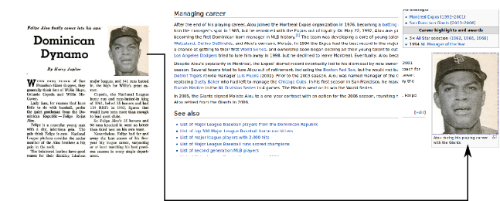
\includegraphics[scale=1]{../tables/cover_bottom.png}
\vspace{2mm}
\caption*{(2) Johnny Callison's image in January 1964 (in-copyright) issue of Baseball Digest, not reused on Wikipedia}
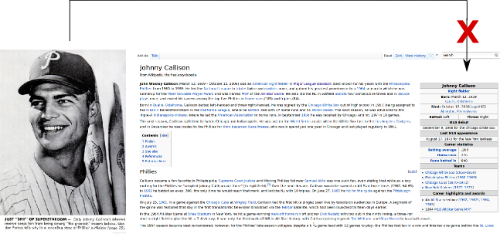
\includegraphics[scale=1]{../tables/cover_top.png}

\end{center}
\begin{quote}
\vspace{5mm}
\end{quote}
\end{figure}

%%% Fig 2: mean charts, digitization
\begin{figure}[!htbp]
\begin{center}
\caption{Citations to Baseball Digest on Wikipedia (Sample A)}
\label{fig:overview}
\caption*{(1) Citations to Baseball Digest before and after Digitization}
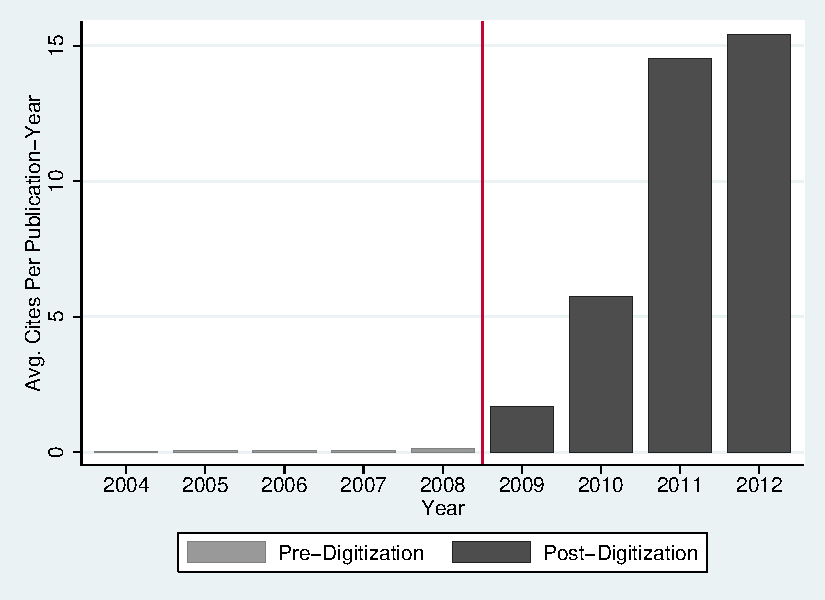
\includegraphics[scale=0.75]{../tables/mean_digit.pdf}
\vspace{5mm}
\caption*{(2) Citations to Baseball Digest for issues published before and after 1964}
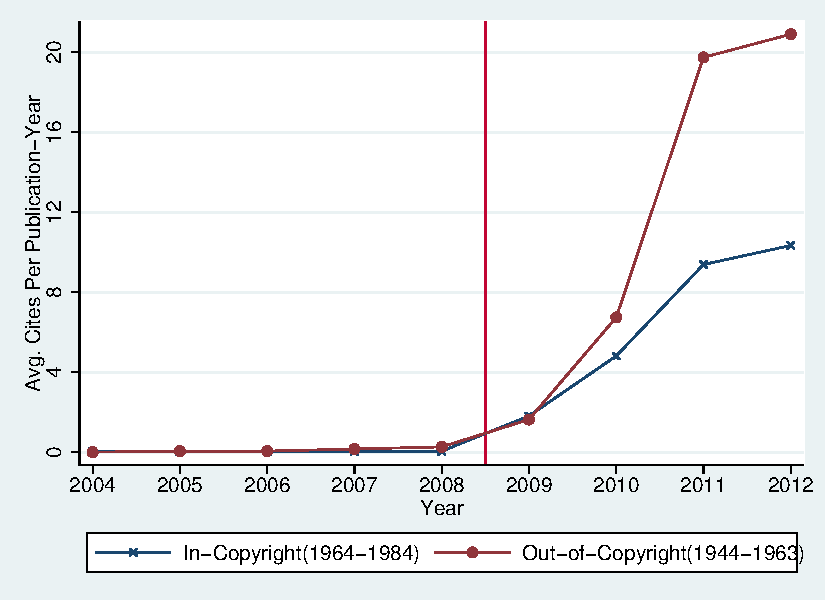
\includegraphics[scale=0.75]{../tables/mean_connected_cites.pdf}
%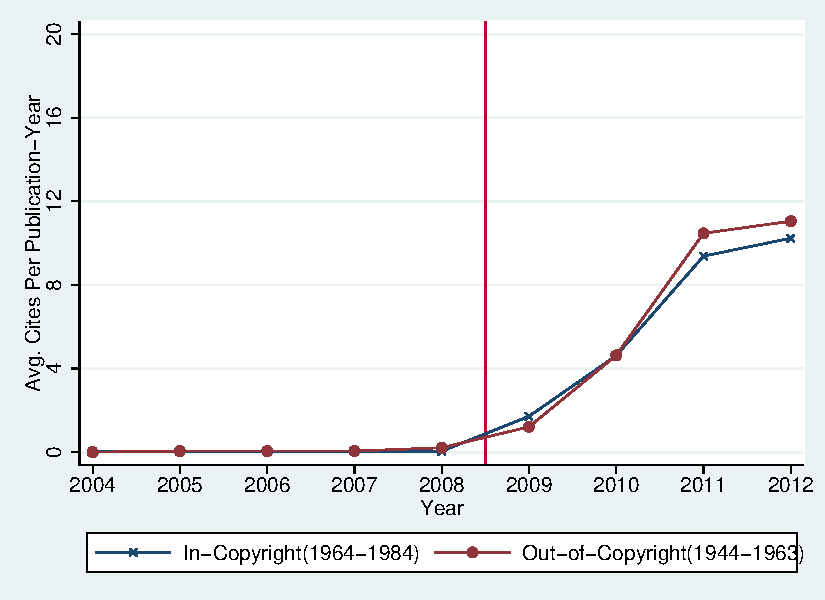
\includegraphics[scale=0.25]{../tables/mean_connected_text.pdf}
%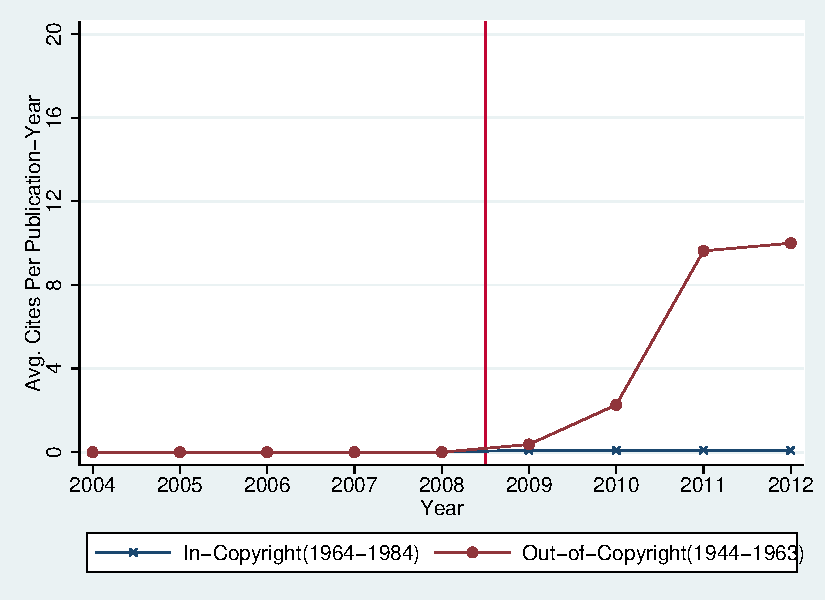
\includegraphics[scale=0.25]{../tables/mean_connected_img.pdf}
\end{center}

\begin{quote}
\emph{Note:} This plot presents some simple descriptive data on citations to Baseball Digest issues. Panel (1) presents average citations per publication-year of Baseball Digest on Wikipedia before and after the Google Books digitization event in 2008. Panel (2) presents similar information, but data are presented separately for all publication-years before 1964 (out-of-copyright) and those in or after 1964 (in-copyright). See text for more detailed data and variable descriptions. 
\end{quote}
\end{figure}

%% Fig 3. DD picture
%\begin{landscape}

\begin{figure}[!htbp]
\begin{center}
\caption{Time-Varying Estimates of the Impact of Copyright\\ on Citations to Baseball Digest}
\label{fig:ddpic}
\caption*{(1) Sample A : Total Citations}
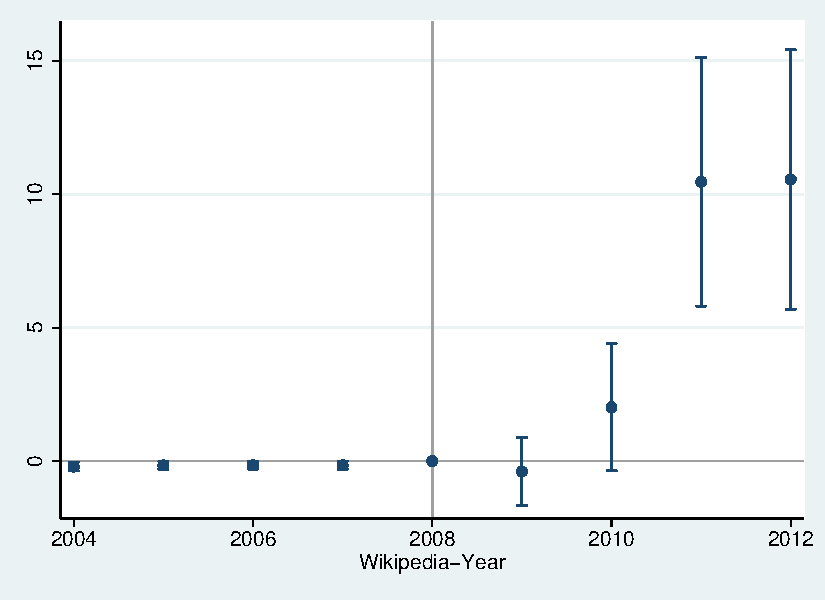
\includegraphics[scale=0.7]{../tables/cite_timeline_cites.pdf}
\vspace{2mm}
\caption*{(2) Sample B : Total Citations}
%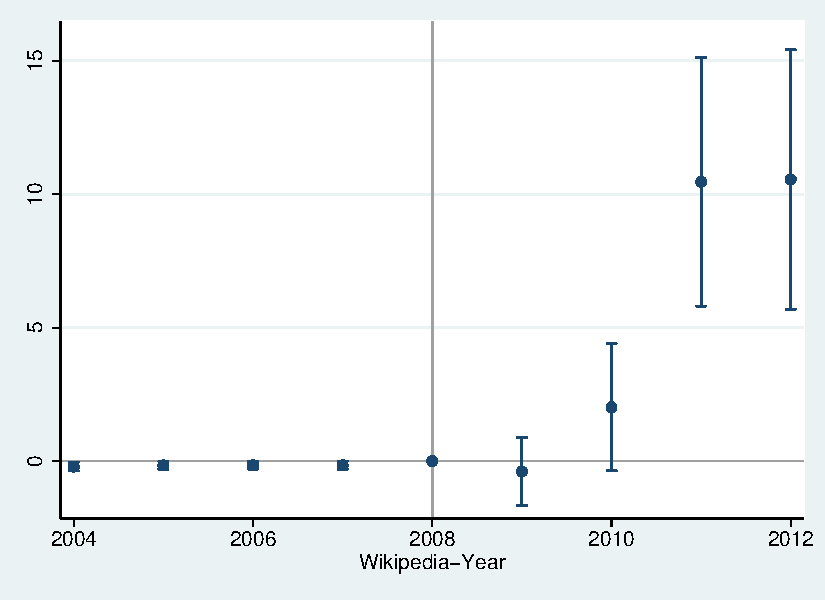
\includegraphics[scale=0.6]{../tables/cite_timeline_cites.pdf}
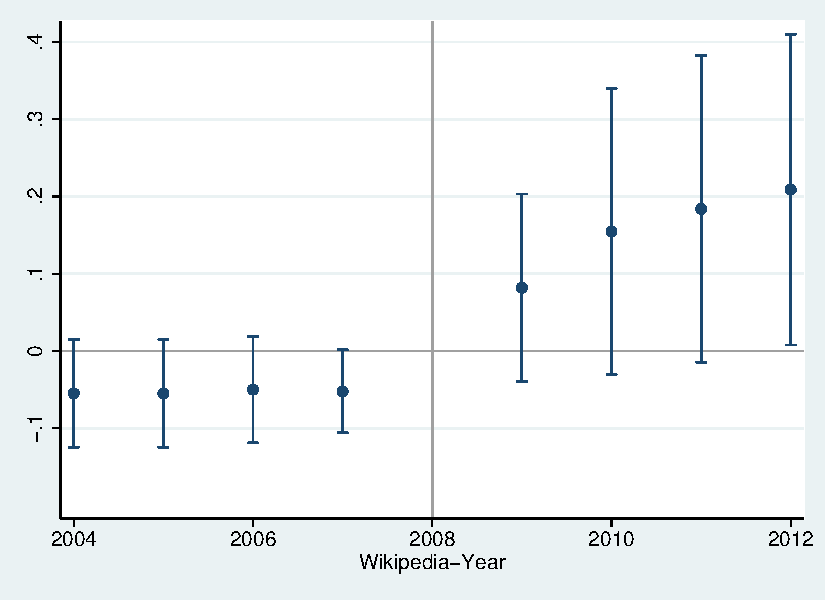
\includegraphics[scale=0.7]{../tables/timeline_bd_1.pdf}

%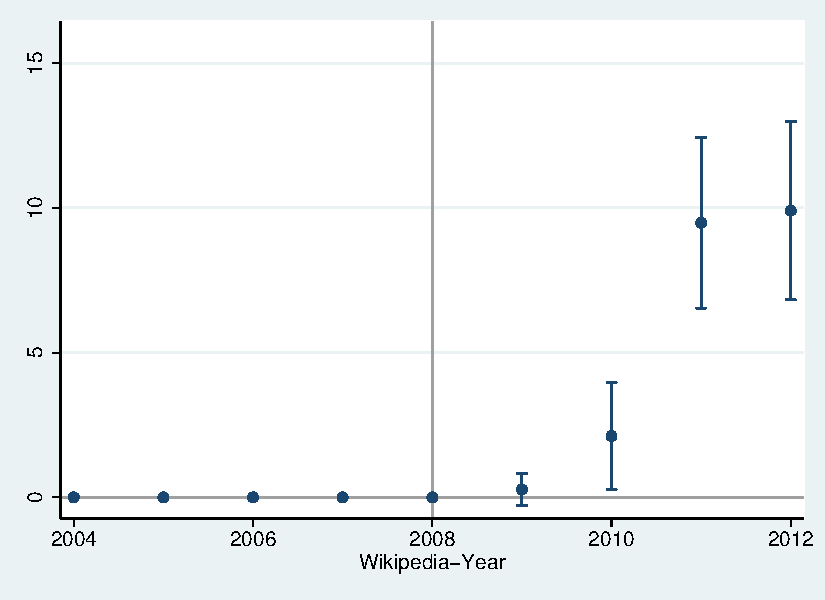
\includegraphics[scale=0.6]{../tables/cite_timeline_img.pdf}
%\vspace{5mm}
%\caption*{Panel B : Basketball Players}
%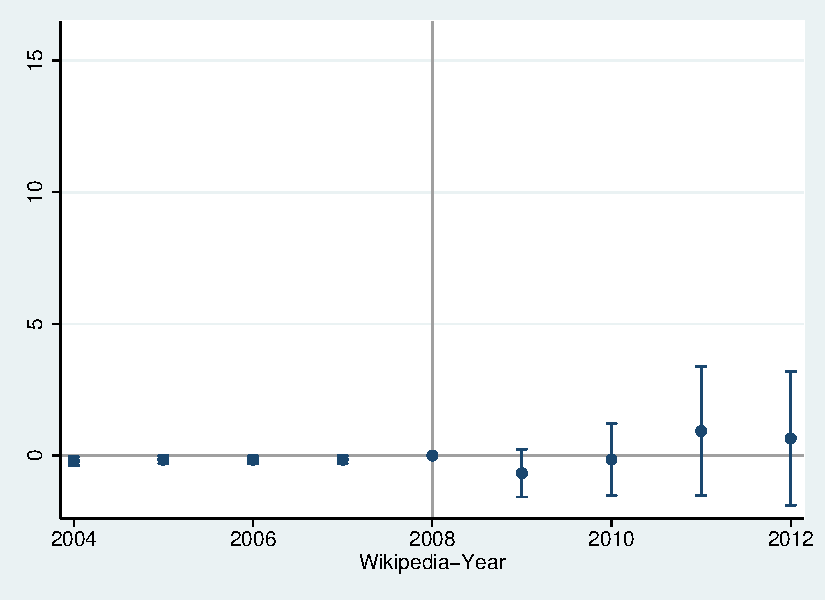
\includegraphics[scale=0.6]{../tables/cite_timeline_text.pdf}
\end{center}

\begin{quote}
%\begin{adjustwidth}{-2cm}{-2cm}
\emph{Note:} This figure plots coefficients (and 95 percent confidence intervals) from the event study specifications described in Section \ref{sec:timevary}. On the $x$ axis is the Wikipedia-year and the reference year is 2008, the year of the digitization event. This specification is based on Sample A for Panel (1) and Sample B for Panel (2), the coefficients are estimates from ordinary-least-squares (OLS) models, and standard errors are clustered. The dependent variable in both panels is the total number of citations in a calendar year. See text for more detailed data and variable descriptions. 
%\end{adjustwidth}

\end{quote}
\end{figure}
%\end{landscape}


%Fig 4. Killer Pic Sample A
%\begin{landscape}

\begin{figure}[!htbp]
\begin{center}
\caption{Citations to Baseball Digest Published Before and After the 1964 Copyright Cutoff (Sample A)}
\label{fig:killer_cite}
%\caption*{Panel A : Citation Gains at the Issue-Year Level between 2012 and 2008}
\vspace{1cm}

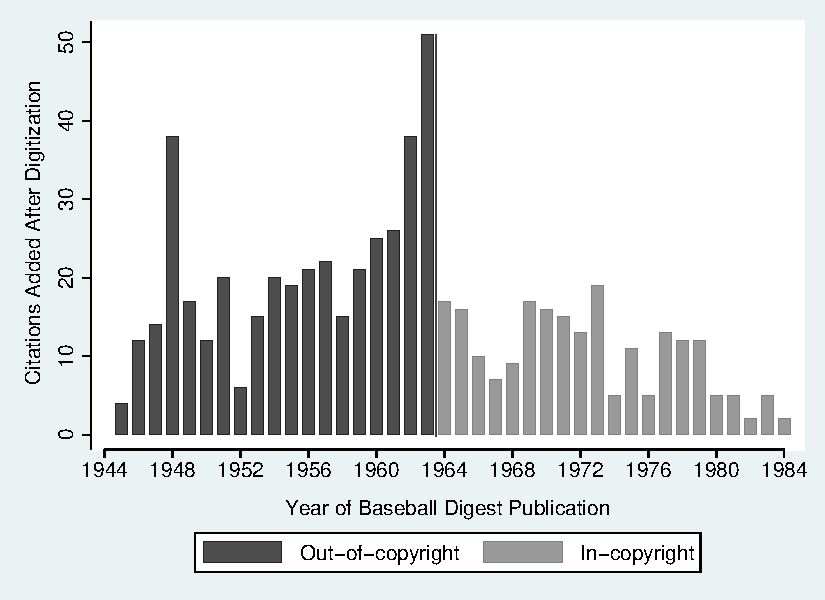
\includegraphics[scale=1]{../tables/cite_killer_cite.pdf}
%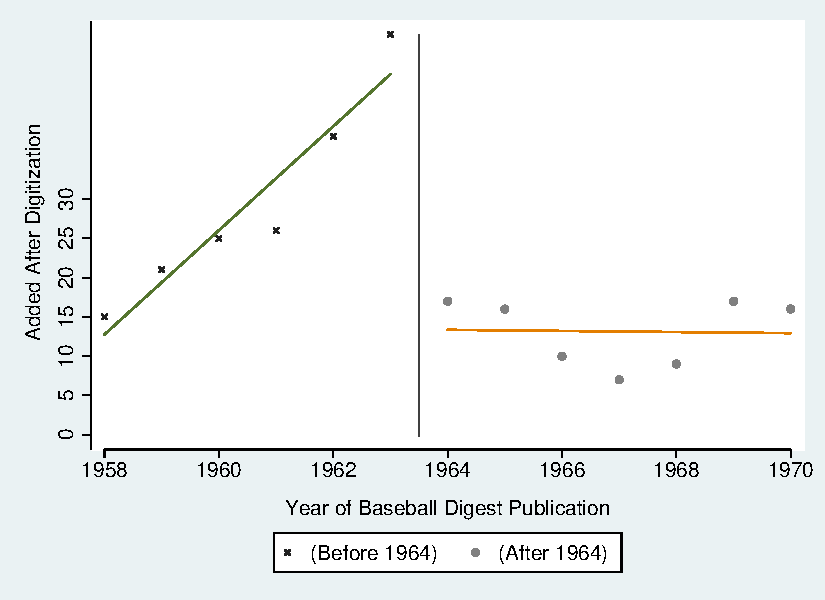
\includegraphics[scale=1]{../tables/cite_scatter_cite.pdf}


%\vspace{2mm}
%\caption*{Panel B : Comparing Citation Gains For Image Reuse and In-Text Citations}
%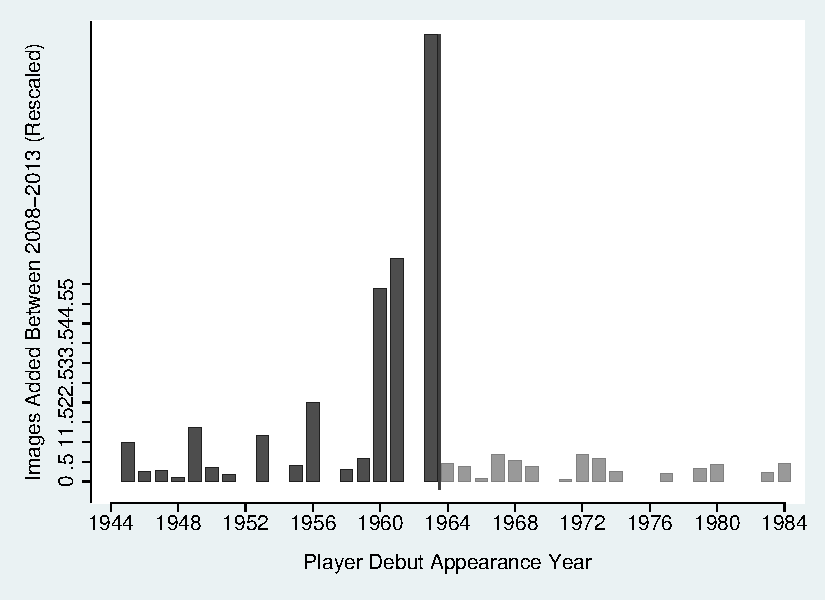
\includegraphics[scale=0.75]{../tables/killerpic2_1_bd.pdf}

%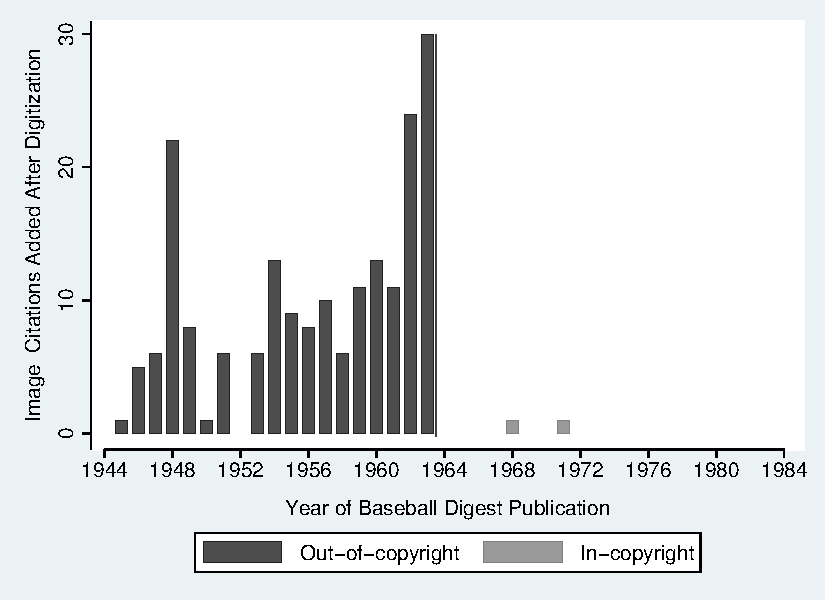
\includegraphics[scale=0.65]{../tables/cite_killer_img.pdf}
%\vspace{5mm}
%\caption*{Panel B : Basketball Players}
%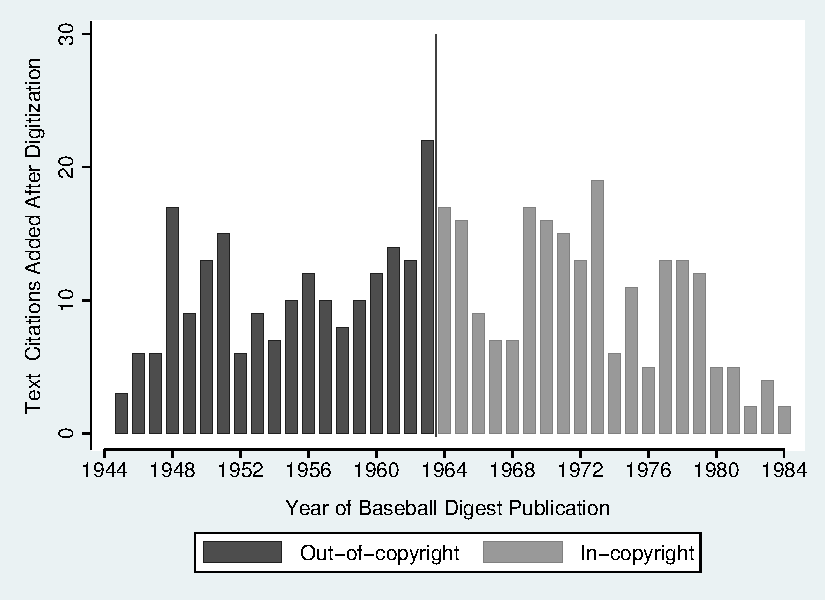
\includegraphics[scale=0.65]{../tables/cite_killer_text.pdf}
\end{center}
\vspace{1cm}
\begin{quote}
%\begin{adjustwidth}{-2cm}{-2cm}
\emph{Note:} This figure plots the growth in citations to Baseball Digest publication-years in 2012 as compared to 2008. Out-of-copyright publication-years (1944-1963) are shown in dark grey, while in-copyright publication-years (1964-1984) are shown in light grey. See text for more detailed data and variable descriptions. 
%\end{adjustwidth}

\end{quote}
\end{figure}
%\end{landscape}

\newpage


%\newpage
%%\begin{landscape}
%%%%% Fig 5. Killer Pic for Images and Text

\newpage
%\begin{landscape}

\begin{figure}[!htbp]
\begin{center}
\caption{Impact of Copyright on Image and Text Citations (Sample A)}
\label{fig:killer_img}
\caption*{(1) Image Citations}

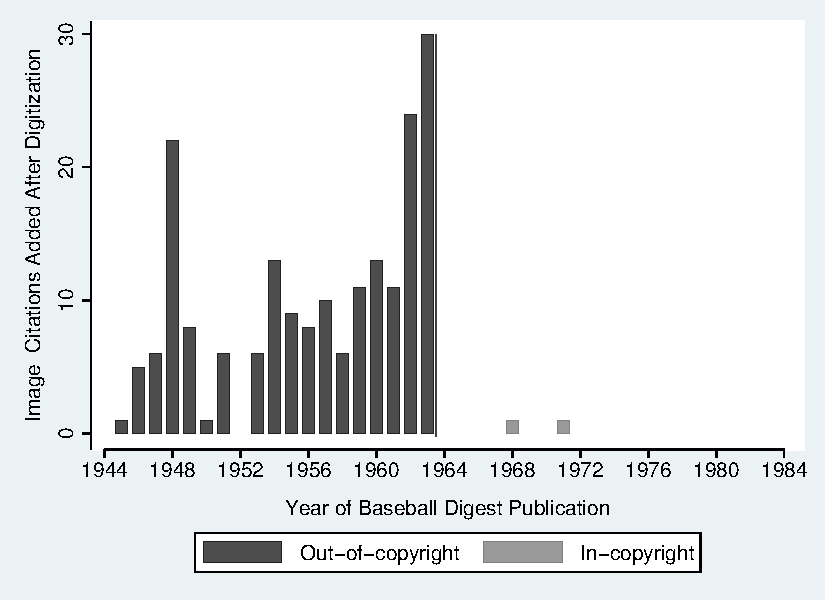
\includegraphics[scale=0.7]{../tables/cite_killer_img.pdf}

\vspace{0.2cm}
\caption*{(2) Text Citations}
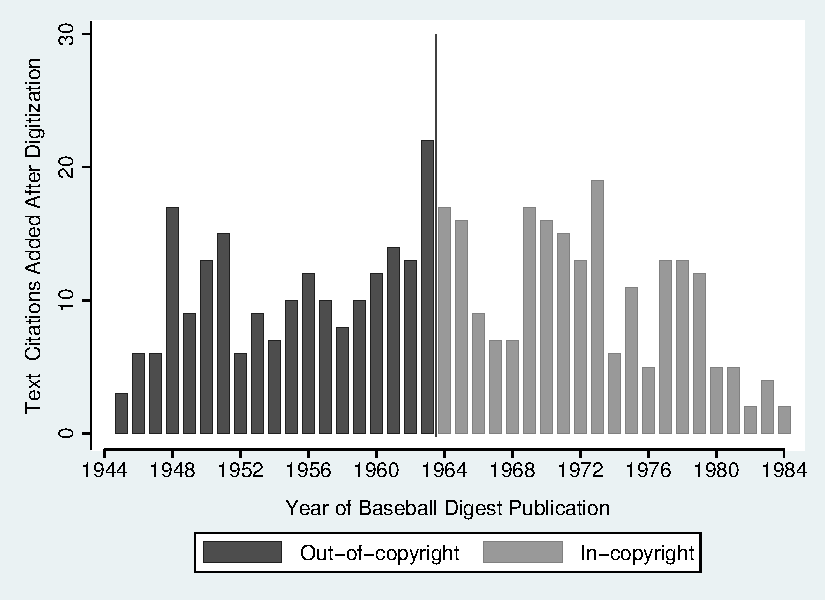
\includegraphics[scale=0.75]{../tables/cite_killer_text.pdf}

%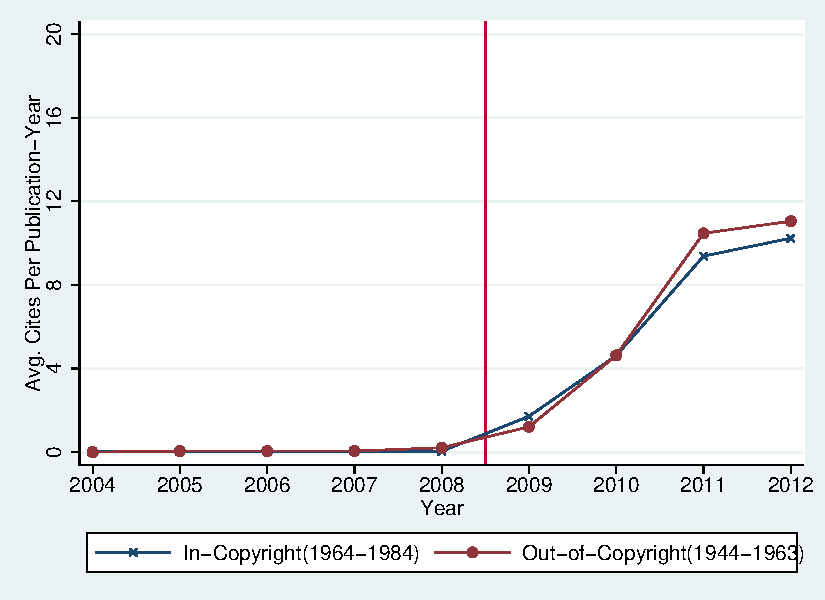
\includegraphics[scale=0.25]{../tables/mean_connected_text.pdf}
%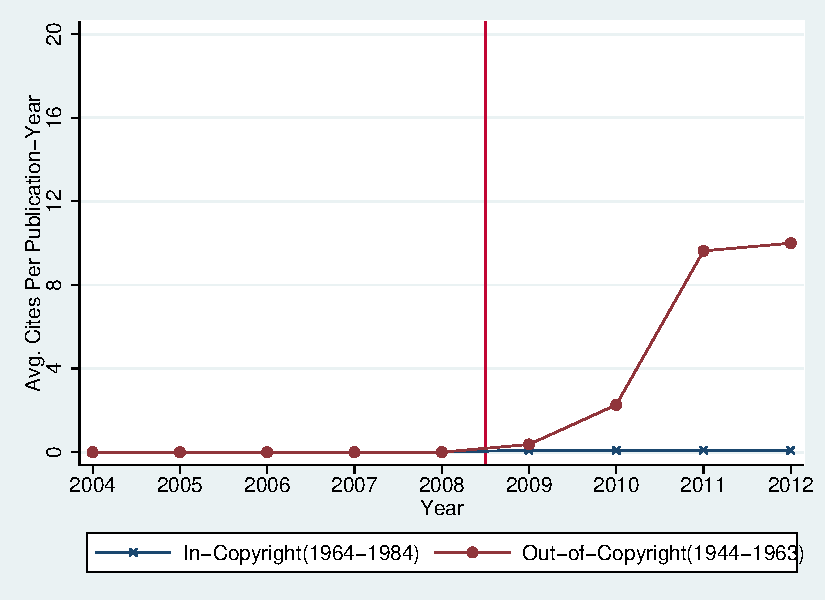
\includegraphics[scale=0.25]{../tables/mean_connected_img.pdf}
\vspace{5mm}

%\caption*{Panel B : Time Varying Estimates of the Impact of Copyright on Wikipedia Pages}
%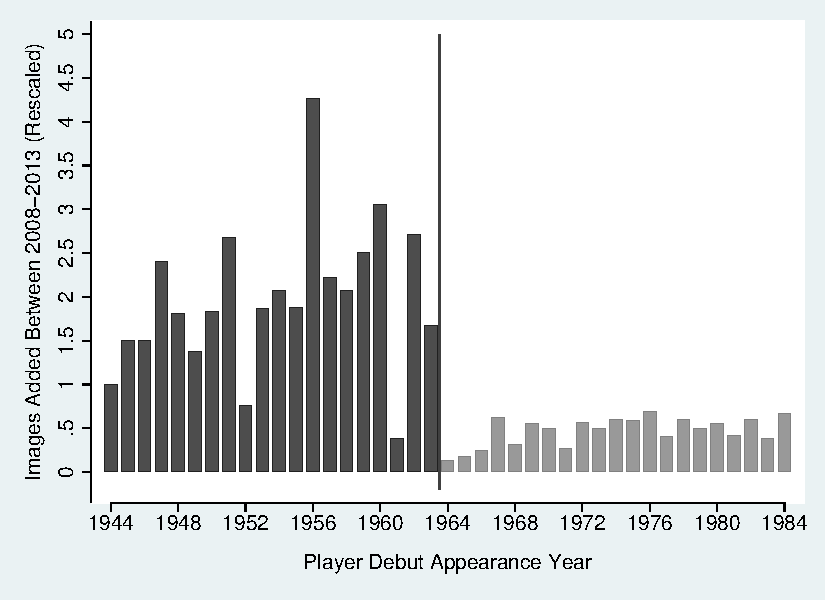
\includegraphics[scale=0.65]{../tables/killerpic2_1_img.pdf}
%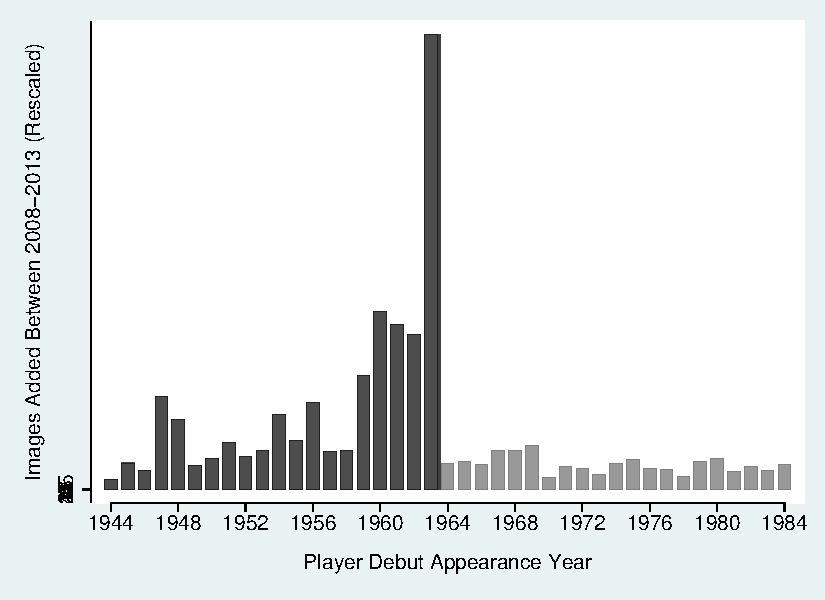
\includegraphics[scale=0.65]{../tables/killerpic2_1_text.pdf}
%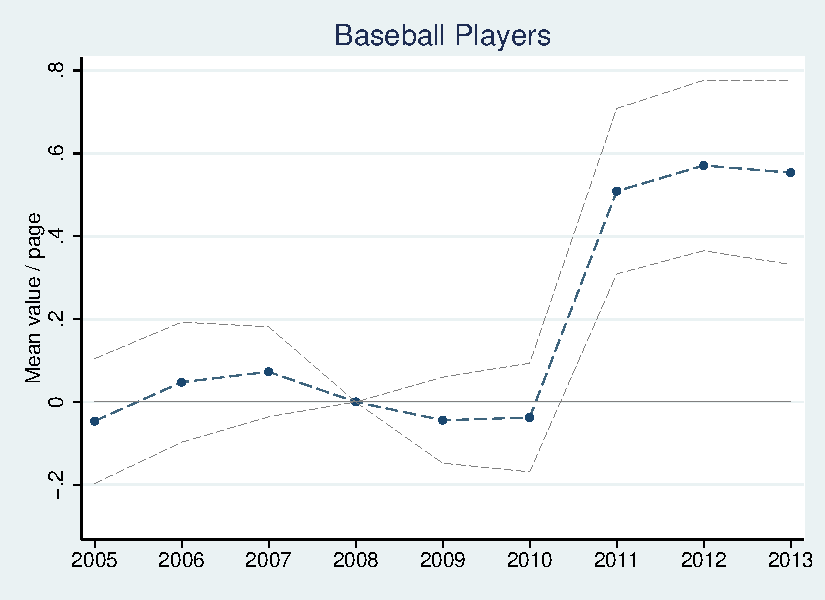
\includegraphics[scale=0.75]{../tables/timeline_img_1.pdf}
%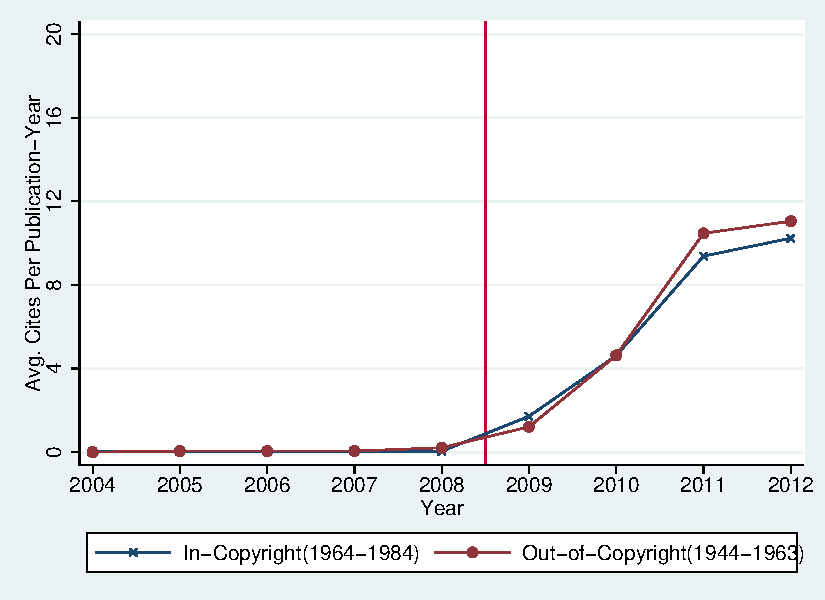
\includegraphics[scale=0.25]{../tables/mean_connected_text.pdf}
%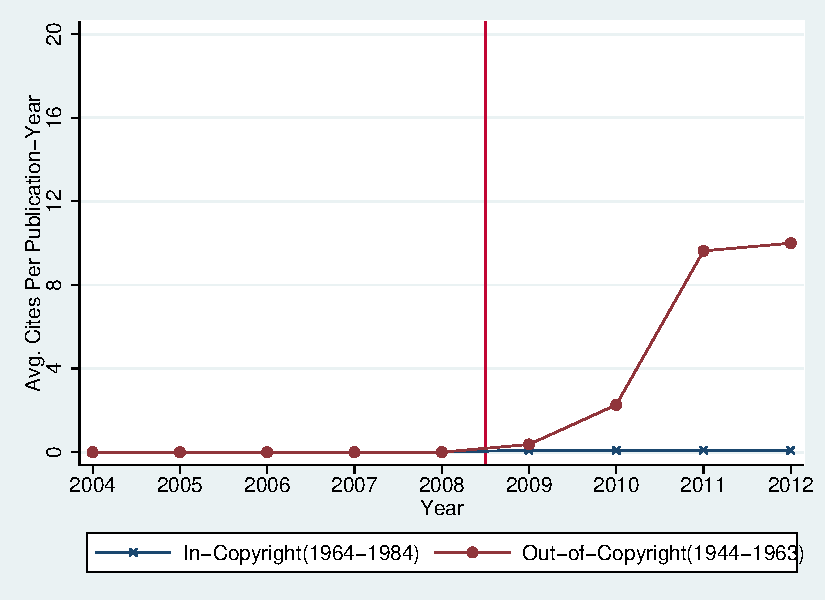
\includegraphics[scale=0.25]{../tables/mean_connected_img.pdf}
\end{center}

\begin{quote}
%\begin{adjustwidth}{-2cm}{-2cm}
%\emph{Note:} This chart documents the impact of the 1964 copyright cutoff for Baseball Digest on the reuse of images and text

\emph{Note:} This figure plots the growth in citations to Baseball Digest publication-years in 2012 as compared to 2008. Panel (1) plots the growth in Image citations, while Panel (2) plots the growth in Text citations. Out-of-copyright publication-years (1944-1963) are shown in dark grey, while in-copyright publication-years (1964-1984) are shown in light grey. See text for more detailed data and variable descriptions. 


%number of images added to baseball Wikipedia pages. Panel A documents the variation in the number of images added between 2008 and 2013 for out-of-copyright (debut before 1964) players and in-copyright (debut after 1964) players. The raw mean is adjusted to account for each player's differing exposure to the copyright rule. Panel B plots coefficients (and 95 percent confidence intervals) from the event study specifications described in Section \ref{sec:timevary}. On the $x$ axis is the calendar year and the reference year is 2008, the year of the digitization event. This specification is based on page-year level observations, the coefficients are estimates from ordinary-least-squares (OLS) models, and standard errors are clustered at the page level. See text for more detailed data and variable descriptions. 
%\end{adjustwidth}
\end{quote}
\end{figure}

%\end{landscape}

%%%%%%%%%%%
%%%%% Fig 6. DD Pic 2 for Images and Text
%%%%%%%%%%%

\begin{figure}[!htbp]
\begin{center}
\caption{Time-Varying Estimates for Image and Text Citations (Sample A)}
\label{fig:ddpic_img}
\caption*{\small{(1) Image Citations}}
%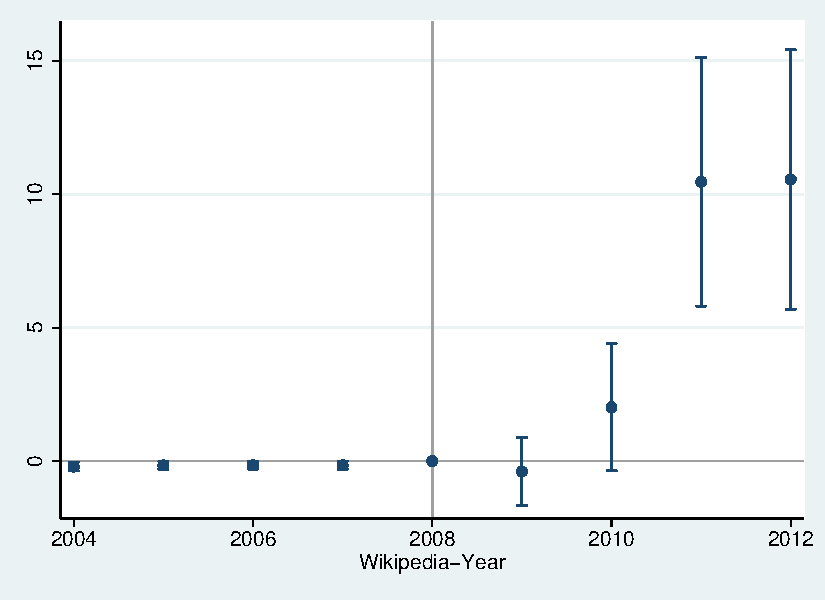
\includegraphics[scale=0.75]{../tables/cite_timeline_cites.pdf}
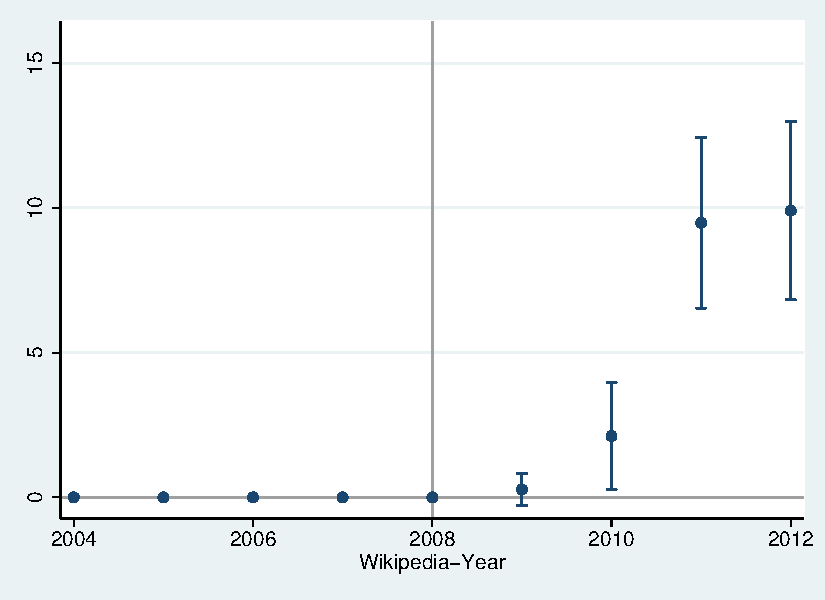
\includegraphics[scale=0.75]{../tables/cite_timeline_img.pdf}

\caption*{\small{(2) Text Citations}}
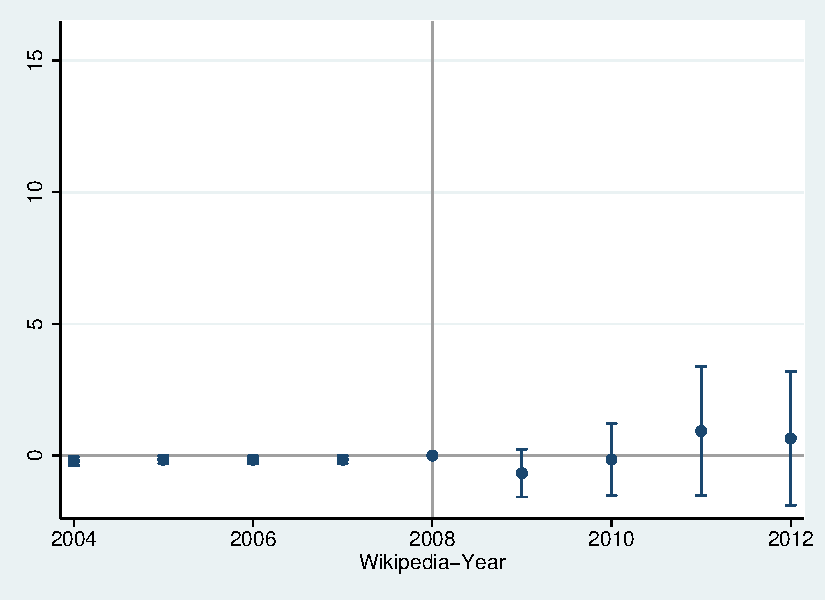
\includegraphics[scale=0.75]{../tables/cite_timeline_text.pdf}
\vspace{2mm}

%\caption*{Sample B : }
%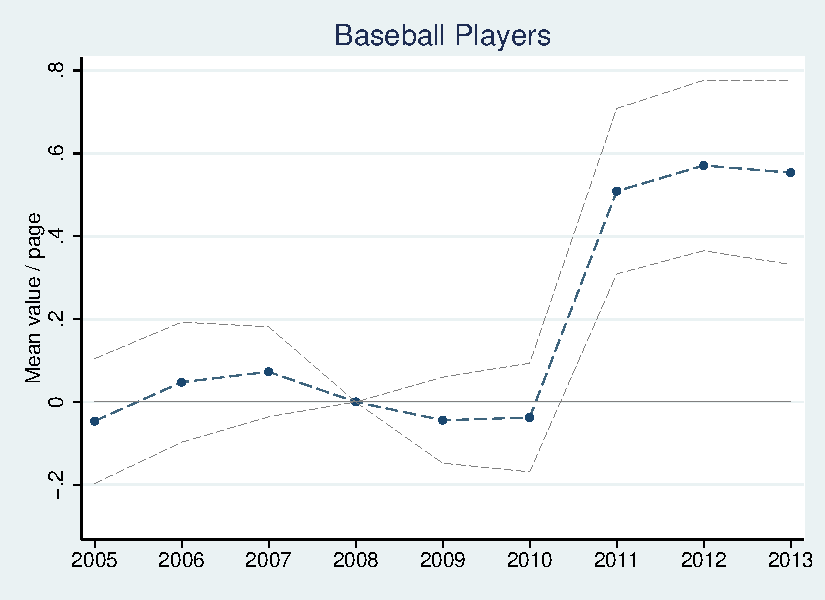
\includegraphics[scale=0.6]{../tables/timeline_img_1.pdf}
%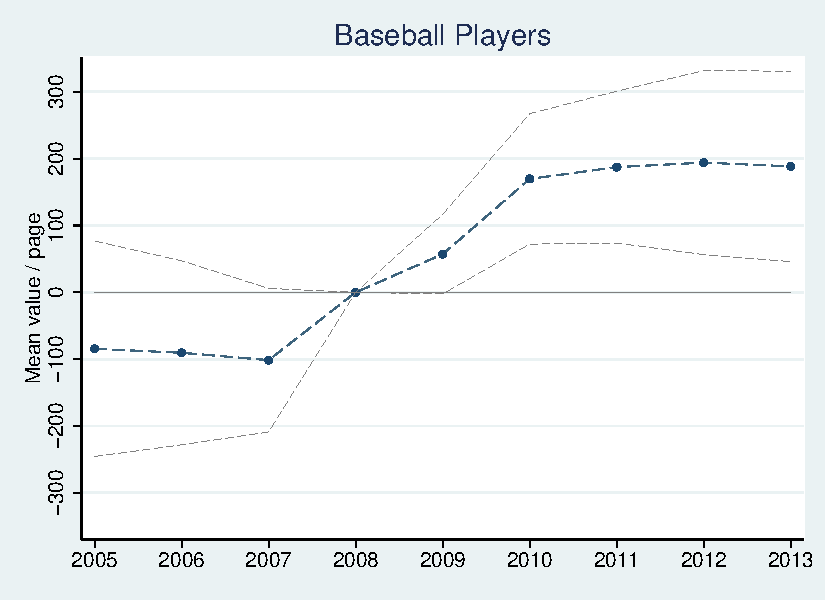
\includegraphics[scale=0.6]{../tables/timeline_text_1.pdf}

%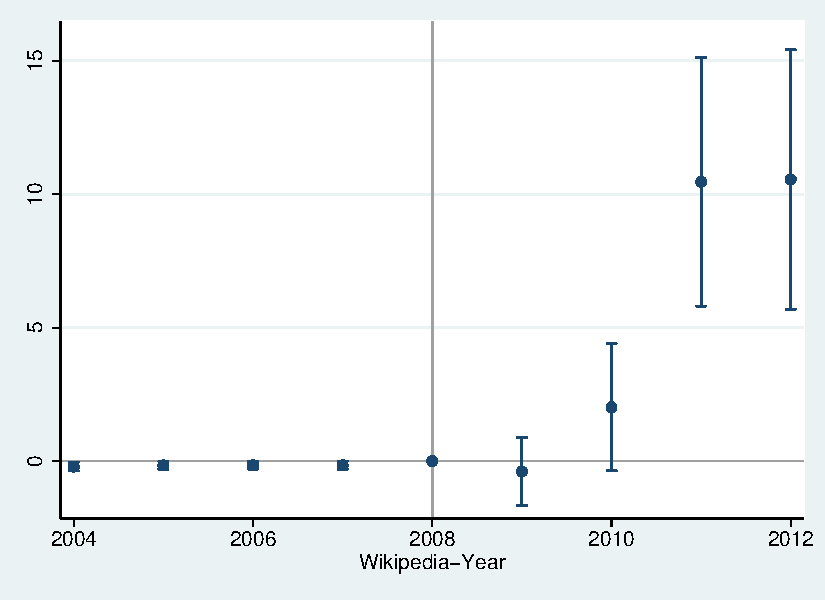
\includegraphics[scale=0.6]{../tables/cite_timeline_cites.pdf}

%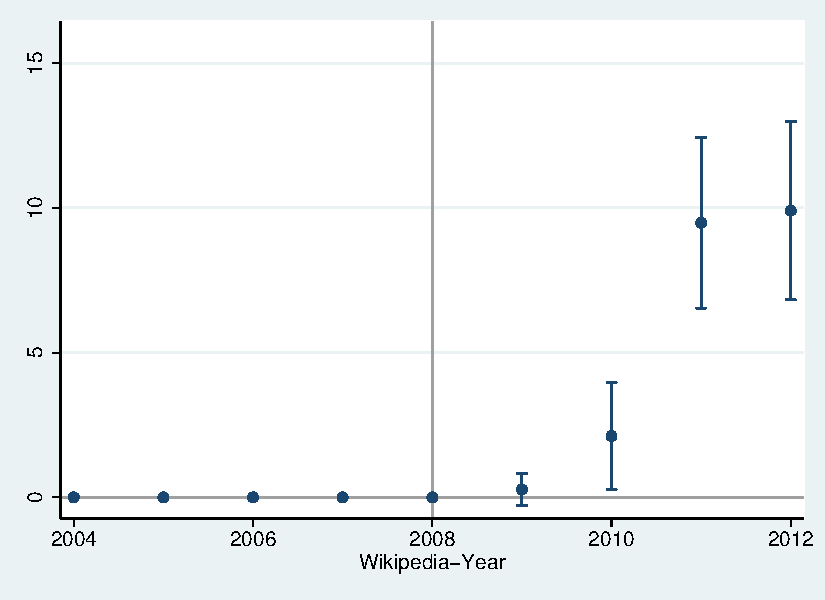
\includegraphics[scale=0.6]{../tables/cite_timeline_img.pdf}
%\vspace{5mm}
%\caption*{Panel B : Basketball Players}
%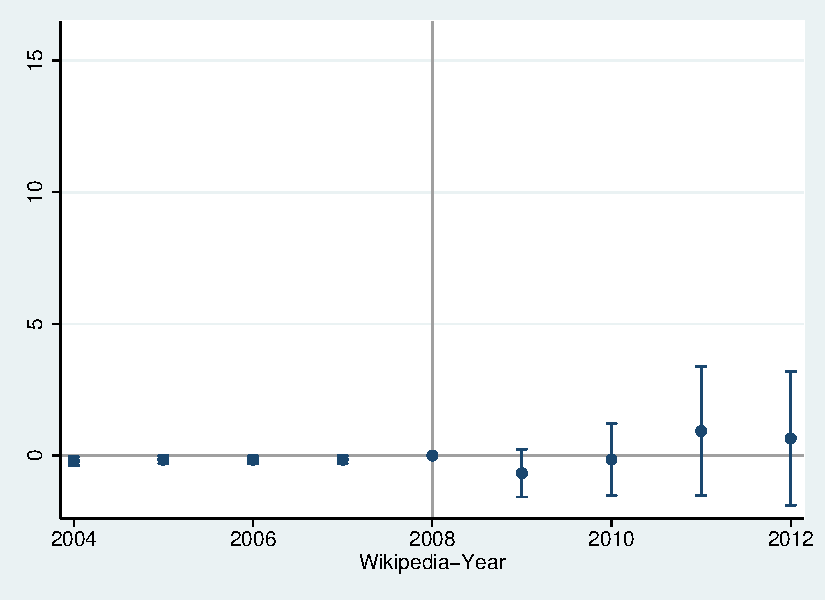
\includegraphics[scale=0.6]{../tables/cite_timeline_text.pdf}
\end{center}

\begin{quote}
\emph{Note:} This figure plots coefficients (and 95 percent confidence intervals) from the event study specifications described in Section \ref{sec:timevary} separately for image (Panel 1) and text citations (Panel 2). On the $x$ axis is the Wikipedia-year and the reference year is 2008, the year of the digitization event. This specification is based on Sample A for Panel (1) and (2). The coefficients are estimated from ordinary-least-squares (OLS) models, and standard errors are clustered. The dependent variable in both panels is the total number of citations in a calendar year. See text for more detailed data and variable descriptions. 

\end{quote}
\end{figure}



%%%%%%%%%%%
%%% Fig 7: HETERO EFFECTS
%%%%%%%%%%%

\begin{figure}[!htbp]
\begin{center}
\caption{Heterogeneous Impacts of Copyright on Wikipedia Pages by Player Quality (Sample B)}
\label{fig:quality}
\vspace{5mm}
\caption*{\small{(1) Images}}
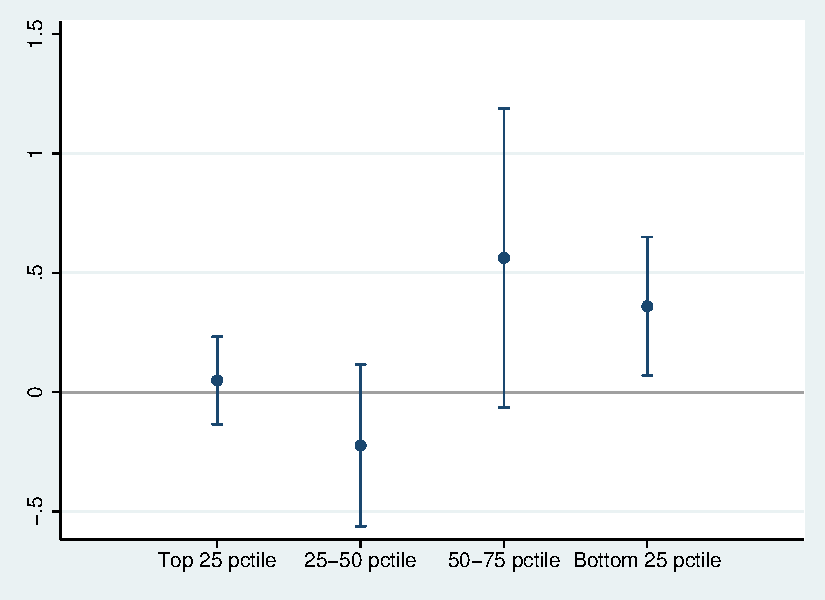
\includegraphics[scale=0.70]{../tables/quality_img.pdf}\\
\vspace{5mm}
\caption*{\small{(2) Traffic}}
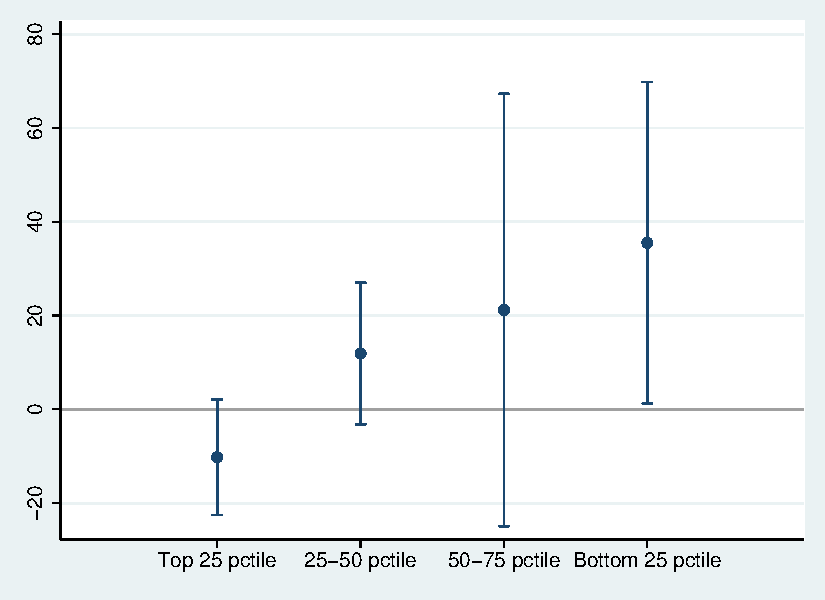
\includegraphics[scale=0.70]{../tables/quality_traf.pdf}

\end{center}
\begin{quote}
%\begin{adjustwidth}{-2cm}{-2cm}
\emph{Note:} This plot documents the differential impact of the Baseball Digest copyright cutoff on baseball player pages of different \emph{quality} as described in Section \ref{sec:diff2}. For this analysis, players are split into 4 different levels of quality based on their percentile rank within the sample of baseball players and the main difference-in-difference estimates are calculated separately for each of the four quality percentiles. Panel (1) plots these estimates for Image Citations, while Panel (2) plots estimates for Traffic. See text for detailed data and variable descriptions.

%%Coefficients ($\beta_3$) are derived from the specification: 

%%$Y_{it} = \alpha + \beta_1 \times post_t \times out-of-copy_i + \beta_2 \times post_t \times quality_i + \beta_3 \times post_t \times out-of-copy_i \times quality_i + \gamma_i+ \delta_t + \epsilon_{it}$ 

%%where $\gamma_{i}$ and $\delta_{t}$ represents player and time fixed effects respectively for player $i$ and year $t$.  All estimates are from ordinary-least-squares (OLS) models. 

%\end{adjustwidth}
\end{quote}
\end{figure}

%%\end{landscape}

%%%%%%%%%%%%%%%% APPENDIX %%%%%%%%%%%%%%%%%%%%%%%%%%%
%blank
%\newpage
%\newpage

\appendix

\setcounter{table}{0}\renewcommand{\thetable}{A.\arabic{table}}
\setcounter{figure}{0}\renewcommand{\thefigure}{A.\arabic{figure}}

%%%%% DD Table %%%%
\begin{center}
\begin{table}[!htbp]
\section{Appendices}

\subsection{Appendix A1 : Robustness Checks}
\label{sec:envelope}

%% BASKETBALL DATA Added

\caption{Estimating the Causal Impact of Digitization}
\vspace{5mm}
{
\def\sym#1{\ifmmode^{#1}\else\(^{#1}\)\fi}
\begin{tabular*}{\hsize}{@{\hskip\tabcolsep\extracolsep\fill}l*{3}{c}}
\toprule
            &\multicolumn{3}{c}{Digitization DD}                              \\\cmidrule(lr){2-4}
            &\multicolumn{1}{c}{Citations}&\multicolumn{1}{c}{Images}&\multicolumn{1}{c}{Text}\\
\midrule
\emph{baseball X post}&       0.340         &       0.459         &       0.391         \\
            &    (0.0494)\sym{***}&    (0.0610)\sym{***}&    (0.0650)\sym{***}\\
\midrule
Player FE   &         Yes         &         Yes         &         Yes         \\
Time FE     &        Year         &        Year         &        Year         \\
adj. $R^2$  &      0.0687         &       0.172         &       0.399         \\
N           &       13260         &       13260         &       13260         \\
Clusters    &        1105         &        1105         &        1105         \\
\bottomrule
\end{tabular*}
}

\begin{quote}
\vspace{5mm}

\emph{+:p$<$0.15; *:p$<$0.10; **:p$<$0.05; ***:p$<$0.01 
\newline
Standard errors clustered at player-level shown in parentheses.}

\vspace{5mm}

\emph{Note:} This table provides estimates that help to determine the causal impact of the Google Books digitization event on reuse. I supplement data in Sample B, with similar data from Wikipedia player-pages for a comparable set of 564 basketball players. The estimates are provided from a difference-in-difference specification where the treatment group is the set of baseball player-pages and the post-period are the years 2009-2012 after the digitization event. All estimates are from ordinary-least-squares (OLS) models. See text for detailed data and variable descriptions.
\end{quote}
\label{tab:basketball}
\end{table}
\end{center}



%%% LEADS - LAGS
\begin{center}
\begin{table}[!htbp]

\caption{Robustness: Exploring pre-trends between in-copyright and out-of-copyright Issues}
%\vspace{5mm}
{\small
{
\def\sym#1{\ifmmode^{#1}\else\(^{#1}\)\fi}
\begin{tabular*}{\hsize}{@{\hskip\tabcolsep\extracolsep\fill}l*{6}{c}}
\toprule
            &\multicolumn{3}{c}{Sample A}                                     &\multicolumn{3}{c}{Sample B}                                     \\\cmidrule(lr){2-4}\cmidrule(lr){5-7}
            &\multicolumn{1}{c}{Citations}&\multicolumn{1}{c}{Images}&\multicolumn{1}{c}{Text}&\multicolumn{1}{c}{Citations}&\multicolumn{1}{c}{Images}&\multicolumn{1}{c}{Text}\\
\midrule
$Digitization_{-3}$&      -0.000         &      -0.000         &      -0.000         &      -0.008         &      -0.194         &      -0.642         \\
            &         (.)         &     (0.000)         &     (0.000)         &     (0.004)\sym{*}  &     (0.024)\sym{***}&     (0.031)\sym{***}\\
\addlinespace
$Digitization_{-2}$&      -0.000         &      -0.000         &      -0.000         &      -0.008         &      -0.075         &      -0.359         \\
            &         (.)         &     (0.000)         &     (0.000)         &     (0.004)\sym{**} &     (0.027)\sym{***}&     (0.022)\sym{***}\\
\addlinespace
$Digitization_{-1}$&      -0.000         &      -0.000         &      -0.000         &      -0.003         &      -0.033         &      -0.106         \\
            &     (0.000)         &     (0.000)         &     (0.000)         &     (0.003)         &     (0.019)\sym{*}  &     (0.009)\sym{***}\\
\addlinespace
$Digitization_{+1}$&       1.762         &       0.095         &       1.667         &       0.046         &       0.060         &       0.088         \\
            &     (0.424)\sym{***}&     (0.066)         &     (0.421)\sym{***}&     (0.015)\sym{***}&     (0.016)\sym{***}&     (0.007)\sym{***}\\
\addlinespace
$Digitization_{+2}$&       4.762         &       0.095         &       4.667         &       0.112         &       0.140         &       0.220         \\
            &     (0.680)\sym{***}&     (0.066)         &     (0.681)\sym{***}&     (0.027)\sym{***}&     (0.020)\sym{***}&     (0.012)\sym{***}\\
\addlinespace
$Digitization_{+3}$&       9.333         &       0.095         &       9.238         &       0.128         &       0.220         &       0.397         \\
            &     (1.064)\sym{***}&     (0.066)         &     (1.060)\sym{***}&     (0.028)\sym{***}&     (0.026)\sym{***}&     (0.017)\sym{***}\\
\addlinespace
$Digitization_{+4}$&      10.286         &       0.095         &      10.190         &       0.132         &       0.259         &       0.472         \\
            &     (1.195)\sym{***}&     (0.066)         &     (1.189)\sym{***}&     (0.028)\sym{***}&     (0.026)\sym{***}&     (0.020)\sym{***}\\
\addlinespace
$Digitization_{-3}$ x out-of-copy&      -0.211         &       0.000         &      -0.211         &      -0.040         &      -0.093         &      -0.180         \\
            &     (0.097)\sym{**} &     (0.000)         &     (0.097)\sym{**} &     (0.027)\sym{+}  &     (0.064)\sym{+}  &     (0.084)\sym{**} \\
\addlinespace
$Digitization_{-2}$ x out-of-copy&      -0.211         &       0.000         &      -0.211         &      -0.037         &      -0.013         &      -0.127         \\
            &     (0.097)\sym{**} &     (0.000)         &     (0.097)\sym{**} &     (0.027)         &     (0.062)         &     (0.067)\sym{*}  \\
\addlinespace
$Digitization_{-1}$ x out-of-copy&      -0.105         &       0.000         &      -0.105         &      -0.035         &       0.033         &      -0.114         \\
            &     (0.073)         &     (0.000)         &     (0.073)         &     (0.021)\sym{*}  &     (0.052)         &     (0.050)\sym{**} \\
\addlinespace
$Digitization_{+1}$ x out-of-copy&      -0.393         &       0.273         &      -0.667         &       0.077         &      -0.038         &       0.050         \\
            &     (0.757)         &     (0.327)         &     (0.544)         &     (0.045)\sym{*}  &     (0.042)         &     (0.024)\sym{**} \\
\addlinespace
$Digitization_{+2}$ x out-of-copy&       1.712         &       2.115         &      -0.404         &       0.160         &      -0.013         &       0.124         \\
            &     (1.443)         &     (1.100)\sym{*}  &     (0.834)         &     (0.068)\sym{**} &     (0.055)         &     (0.039)\sym{***}\\
\addlinespace
$Digitization_{+3}$ x out-of-copy&      10.140         &       9.484         &       0.657         &       0.187         &       0.383         &       0.101         \\
            &     (2.762)\sym{***}&     (1.748)\sym{***}&     (1.453)         &     (0.073)\sym{**} &     (0.083)\sym{***}&     (0.046)\sym{**} \\
\addlinespace
$Digitization_{+4}$ x out-of-copy&      10.346         &       9.905         &       0.441         &       0.206         &       0.454         &       0.117         \\
            &     (2.938)\sym{***}&     (1.826)\sym{***}&     (1.581)         &     (0.074)\sym{***}&     (0.086)\sym{***}&     (0.055)\sym{**} \\
\midrule
Player FE   &         Yes         &         Yes         &         Yes         &         Yes         &         Yes         &         Yes         \\
Time FE     &        Year         &        Year         &        Year         &        Year         &        Year         &        Year         \\
adj. $R^2$  &       0.748         &       0.573         &       0.799         &       0.043         &       0.134         &       0.365         \\
N           &     360.000         &     360.000         &     360.000         &    9945.000         &    9945.000         &    9945.000         \\
\bottomrule
\end{tabular*}
}

}
\begin{quote}
\vspace{5mm}

\emph{+:p$<$0.15; *:p$<$0.10; **:p$<$0.05; ***:p$<$0.01 
\newline
Standard errors clustered at player-level shown in parentheses.}

\vspace{5mm}

%\emph{Note:} This table presents XXX
\end{quote}
\label{tab:leads_lags}
\end{table}
\end{center}

%%% Falsitifction
\begin{center}
\begin{table}[!htbp]

\caption{Falsification Check -- Alternate Treatment Years}
\vspace{5mm}
%{
\def\sym#1{\ifmmode^{#1}\else\(^{#1}\)\fi}
\begin{tabular*}{\hsize}{@{\hskip\tabcolsep\extracolsep\fill}l*{6}{c}}
\toprule
            &\multicolumn{3}{c}{Sample A}                                     &\multicolumn{3}{c}{Sample B}                                     \\\cmidrule(lr){2-4}\cmidrule(lr){5-7}
            &\multicolumn{1}{c}{Citations}&\multicolumn{1}{c}{Images}&\multicolumn{1}{c}{Text}&\multicolumn{1}{c}{Citations}&\multicolumn{1}{c}{Images}&\multicolumn{1}{c}{Text}\\
\midrule
\emph{out-of-copy X post}&    -0.00835         &      0.0911         &     -0.0994         &      0.0631         &      0.0631         &      0.0631         \\
            &     (0.266)         &     (0.108)         &     (0.195)         &    (0.0398)         &    (0.0398)         &    (0.0398)         \\
\midrule
Player FE   &         Yes         &         Yes         &         Yes         &         Yes         &         Yes         &         Yes         \\
Time FE     &        Year         &        Year         &        Year         &        Year         &        Year         &        Year         \\
adj. $R^2$  &       0.320         &      0.0314         &       0.385         &      0.0350         &      0.0350         &      0.0350         \\
N           &         240         &         240         &         240         &        3246         &        3246         &        3246         \\
\bottomrule
\end{tabular*}
}

{
\def\sym#1{\ifmmode^{#1}\else\(^{#1}\)\fi}
\begin{tabular*}{\hsize}{@{\hskip\tabcolsep\extracolsep\fill}l*{6}{c}}
\toprule
            &\multicolumn{3}{c}{Sample A}                                     &\multicolumn{3}{c}{Sample B}                                     \\\cmidrule(lr){2-4}\cmidrule(lr){5-7}
            &\multicolumn{1}{c}{Cites}&\multicolumn{1}{c}{Cites}&\multicolumn{1}{c}{Log-Cites}&\multicolumn{1}{c}{Cites}&\multicolumn{1}{c}{Cites}&\multicolumn{1}{c}{Log-Cites}\\
\midrule
\emph{out-of-copy X post}&     -0.0209         &    -0.00835         &     -0.0105         &      0.0685         &      0.0631         &      0.0207         \\
            &     (0.296)         &     (0.266)         &    (0.0768)         &    (0.0323)\sym{**} &    (0.0398)         &    (0.0145)         \\
\midrule
Unit of Obs. FE&          No         &         Yes         &         Yes         &          No         &         Yes         &         Yes         \\
Year FE     &         Yes         &         Yes         &         Yes         &         Yes         &         Yes         &         Yes         \\
adj. $R^2$  &       0.256         &       0.320         &       0.541         &      0.0265         &      0.0350         &      0.0441         \\
N           &         240         &         240         &         240         &        3246         &        3246         &        3246         \\
\bottomrule
\end{tabular*}
}

\begin{quote}
\vspace{5mm}

\emph{+:p$<$0.15; *:p$<$0.10; **:p$<$0.05; ***:p$<$0.01 
\newline
Standard errors clustered at player-level shown in parentheses.}

\vspace{5mm}

\emph{Note:} This table presents a falsification check of the baseline specification. In this regression, the panel is restricted to years 2004 to 2009, and the treatment year is assumed to be 2007 rather than 2009. The $out-of-copy$ variable is defined as before, and unit-of-observation fixed effects and time fixed effects are included as indicated. Please see text for detailed data and variable descriptions. 
\end{quote}
\label{tab:false}
\end{table}
\end{center}

%%%%% alternate years

%%% Falsitifction
\begin{center}
\begin{table}[!htbp]

\caption{Robustness Check : Adding Panel Restrictions}
\vspace{5mm}
\caption*{(1) Wikipedia-Years 2005-2011}
%{
\def\sym#1{\ifmmode^{#1}\else\(^{#1}\)\fi}
\begin{tabular*}{\hsize}{@{\hskip\tabcolsep\extracolsep\fill}l*{6}{c}}
\toprule
            &\multicolumn{3}{c}{Sample A}                                     &\multicolumn{3}{c}{Sample B}                                     \\\cmidrule(lr){2-4}\cmidrule(lr){5-7}
            &\multicolumn{1}{c}{Citations}&\multicolumn{1}{c}{Images}&\multicolumn{1}{c}{Text}&\multicolumn{1}{c}{Citations}&\multicolumn{1}{c}{Images}&\multicolumn{1}{c}{Text}\\
\midrule
\emph{out-of-copy X post}&       4.148         &       3.992         &       0.156         &       0.180         &       0.180         &       0.180         \\
            &     (1.455)\sym{***}&     (0.884)\sym{***}&     (0.858)         &     (0.102)\sym{*}  &     (0.102)\sym{*}  &     (0.102)\sym{*}  \\
\midrule
Player FE   &         Yes         &         Yes         &         Yes         &         Yes         &         Yes         &         Yes         \\
Time FE     &        Year         &        Year         &        Year         &        Year         &        Year         &        Year         \\
adj. $R^2$  &       0.685         &       0.363         &       0.797         &      0.0695         &      0.0695         &      0.0695         \\
N           &         280         &         280         &         280         &        3787         &        3787         &        3787         \\
\bottomrule
\end{tabular*}
}

{
\def\sym#1{\ifmmode^{#1}\else\(^{#1}\)\fi}
\begin{tabular*}{\hsize}{@{\hskip\tabcolsep\extracolsep\fill}l*{6}{c}}
\toprule
            &\multicolumn{3}{c}{Sample A}                                     &\multicolumn{3}{c}{Sample B}                                     \\\cmidrule(lr){2-4}\cmidrule(lr){5-7}
            &\multicolumn{1}{c}{Cites}&\multicolumn{1}{c}{Cites}&\multicolumn{1}{c}{Log-Cites}&\multicolumn{1}{c}{Cites}&\multicolumn{1}{c}{Cites}&\multicolumn{1}{c}{Log-Cites}\\
\midrule
\emph{out-of-copy X post}&       4.035         &       3.951         &       0.198         &       0.199         &       0.180         &      0.0655         \\
            &     (1.487)\sym{***}&     (1.459)\sym{***}&     (0.150)         &    (0.0657)\sym{***}&     (0.102)\sym{*}  &    (0.0345)\sym{*}  \\
\midrule
Unit of Obs. FE&          No         &         Yes         &         Yes         &          No         &         Yes         &         Yes         \\
Year FE     &         Yes         &         Yes         &         Yes         &         Yes         &         Yes         &         Yes         \\
adj. $R^2$  &       0.619         &       0.678         &       0.889         &      0.0444         &      0.0695         &      0.0898         \\
N           &         280         &         280         &         280         &        3787         &        3787         &        3787         \\
\bottomrule
\end{tabular*}
}

\vspace{5mm}
\caption*{(2) Wikipedia-Years 2006-2010}
{
\def\sym#1{\ifmmode^{#1}\else\(^{#1}\)\fi}
\begin{tabular*}{\hsize}{@{\hskip\tabcolsep\extracolsep\fill}l*{6}{c}}
\toprule
            &\multicolumn{3}{c}{Sample A}                                     &\multicolumn{3}{c}{Sample B}                                     \\\cmidrule(lr){2-4}\cmidrule(lr){5-7}
            &\multicolumn{1}{c}{Cites}&\multicolumn{1}{c}{Cites}&\multicolumn{1}{c}{Log-Cites}&\multicolumn{1}{c}{Cites}&\multicolumn{1}{c}{Cites}&\multicolumn{1}{c}{Log-Cites}\\
\midrule
\emph{out-of-copy X post}&       0.875         &       0.764         &     -0.0325         &       0.177         &       0.152         &      0.0540         \\
            &     (0.984)         &     (0.960)         &     (0.159)         &    (0.0745)\sym{**} &    (0.0914)\sym{*}  &    (0.0316)\sym{*}  \\
\midrule
Unit of Obs. FE&          No         &         Yes         &         Yes         &          No         &         Yes         &         Yes         \\
Year FE     &         Yes         &         Yes         &         Yes         &         Yes         &         Yes         &         Yes         \\
adj. $R^2$  &       0.478         &       0.570         &       0.820         &      0.0381         &      0.0595         &      0.0757         \\
N           &         200         &         200         &         200         &        2705         &        2705         &        2705         \\
\bottomrule
\end{tabular*}
}

%{
\def\sym#1{\ifmmode^{#1}\else\(^{#1}\)\fi}
\begin{tabular*}{\hsize}{@{\hskip\tabcolsep\extracolsep\fill}l*{6}{c}}
\toprule
            &\multicolumn{3}{c}{Sample A}                                     &\multicolumn{3}{c}{Sample B}                                     \\\cmidrule(lr){2-4}\cmidrule(lr){5-7}
            &\multicolumn{1}{c}{Citations}&\multicolumn{1}{c}{Images}&\multicolumn{1}{c}{Text}&\multicolumn{1}{c}{Citations}&\multicolumn{1}{c}{Images}&\multicolumn{1}{c}{Text}\\
\midrule
\emph{out-of-copy X post}&       0.917         &       1.221         &      -0.303         &       0.152         &       0.152         &       0.152         \\
            &     (0.945)         &     (0.620)\sym{*}  &     (0.641)         &    (0.0914)\sym{*}  &    (0.0914)\sym{*}  &    (0.0914)\sym{*}  \\
\midrule
Player FE   &         Yes         &         Yes         &         Yes         &         Yes         &         Yes         &         Yes         \\
Time FE     &        Year         &        Year         &        Year         &        Year         &        Year         &        Year         \\
adj. $R^2$  &       0.580         &       0.113         &       0.710         &      0.0595         &      0.0595         &      0.0595         \\
N           &         200         &         200         &         200         &        2705         &        2705         &        2705         \\
\bottomrule
\end{tabular*}
}

\begin{quote}
\vspace{5mm}

\emph{p$<$0.10; **:p$<$0.05; ***:p$<$0.01 
\newline
Standard errors clustered at player-level shown in parentheses.}

\vspace{5mm}

\emph{Note:} This table presents robustness checks for the baseline specification to alternate panel restrictions. The specification is similar to the baseline specification and is estimated using OLS. However, instead of using the complete panel from 2004-2012, Panel (1) only includes data from years 2005-2011, and Panel (2) includes data from year 2006-2010. The $out-of-copy$ and $post$ variables are defined as before, and unit-of-observation fixed effects and time fixed effects are included as indicated. Please see text for detailed data and variable descriptions. 
\end{quote}
\label{tab:short_timeline}
\end{table}
\end{center}


%%%%%%%%%%%%%% ALT SPEC

\begin{center}
\begin{table}[!htbp]

\caption{Robustness to Sample Restrictions, Alternate Variables \\ and Treatment Definition (Sample B)}
\vspace{5mm}
\begin{adjustwidth}{.2cm}{.2cm}
{
\def\sym#1{\ifmmode^{#1}\else\(^{#1}\)\fi}
\begin{tabular*}{\hsize}{@{\hskip\tabcolsep\extracolsep\fill}l*{4}{c}}
\toprule
                                                  &\multicolumn{1}{c}{(1)}&\multicolumn{1}{c}{(2)}&\multicolumn{1}{c}{(3)}&\multicolumn{1}{c}{(4)}\\
\midrule \underline{\textbf{Panel A: Citations}} \vspace{5mm}\\
\emph{out-of-copy X post}                         &      0.0359         &      0.0845         &      0.0434         &      0.0517         \\
                                                  &    (0.0429)         &    (0.0340)\sym{**} &    (0.0306)         &    (0.0253)\sym{**} \\

\end{tabular*} }
{
\def\sym#1{\ifmmode^{#1}\else\(^{#1}\)\fi}
\begin{tabular*}{\hsize}{@{\hskip\tabcolsep\extracolsep\fill}l*{4}{c}}
\midrule \vspace{5mm} \underline{\textbf{Panel B : Images}}\hphantom{ons}\vspace{5mm}\\
\emph{out-of-copy X post}                         &       0.570         &       0.717         &       0.203         &     0.00904         \\
                                                  &     (0.244)\sym{**} &     (0.166)\sym{***}&     (0.128)\sym{+}  &    (0.0309)         \\

\end{tabular*} }
{
\def\sym#1{\ifmmode^{#1}\else\(^{#1}\)\fi}
\begin{tabular*}{\hsize}{@{\hskip\tabcolsep\extracolsep\fill}l*{4}{c}}
\midrule \vspace{5mm} \underline{\textbf{Panel C : Text}}\hphantom{ations}\vspace{5mm}\\
\emph{out-of-copy X post}                         &       0.238         &       0.509         &       0.261         &      1779.0         \\
                                                  &     (0.227)         &     (0.158)\sym{***}&     (0.121)\sym{**} &     (812.7)\sym{**} \\
\midrule
 FE                                               &         Yes         &         Yes         &         Yes         &         Yes         \\
Time FE                                           &        Year         &        Year         &        Year         &        Year         \\
N                                                 &        3438         &        4869         &        3663         &        4398         \\
Adj R-square                                      &       0.421         &       0.406         &       0.417         &       0.360         \\
\bottomrule
\end{tabular*}
}

%{
\def\sym#1{\ifmmode^{#1}\else\(^{#1}\)\fi}
\begin{tabular*}{\hsize}{@{\hskip\tabcolsep\extracolsep\fill}l*{2}{c}}
\toprule
                                                  &\multicolumn{1}{c}{OLS}&\multicolumn{1}{c}{OLS}\\
\midrule \makebox[13em][l]{\underline{\textbf{Panel A: Citations}} \vspace{5mm}}\\
\emph{out-of-copy X post}                         &      0.0965         &       3.924         \\
                                                  &    (0.0447)\sym{**} &     (1.207)\sym{***}\\

\end{tabular*} }
{
\def\sym#1{\ifmmode^{#1}\else\(^{#1}\)\fi}
\begin{tabular*}{\hsize}{@{\hskip\tabcolsep\extracolsep\fill}l*{2}{c}}
\midrule \vspace{5mm} \makebox[13em][l]{\underline{\textbf{Panel B : Images}}\vspace{5mm} ($\bar{y}$=4.19)}\\
\emph{out-of-copy X post}                         &           0         &       3.647         \\
                                                  &         (.)         &     (0.729)\sym{***}\\

\end{tabular*} }
{
\def\sym#1{\ifmmode^{#1}\else\(^{#1}\)\fi}
\begin{tabular*}{\hsize}{@{\hskip\tabcolsep\extracolsep\fill}l*{2}{c}}
\midrule \vspace{5mm} \makebox[13em][l]{\underline{\textbf{Panel C : Text}}\vspace{5mm} ($\bar{y}$=4.19)}\\
\emph{out-of-copy X post}                         &      0.0965         &       0.277         \\
                                                  &    (0.0447)\sym{**} &     (0.681)         \\
\midrule
Issue-Year FE                                     &         Yes         &         Yes         \\
Time FE                                           &        Year         &        Year         \\
N                                                 &         200         &         360         \\
Adj R-square                                      &      0.0837         &       0.812         \\
\bottomrule
\end{tabular*}
}

\end{adjustwidth}

\begin{quote}
\vspace{5mm}

\emph{+:p$<$0.15; *:p$<$0.10; **:p$<$0.05; ***:p$<$0.01 
\newline
Standard errors clustered at player-level shown in parentheses.}
\vspace{5mm}

\emph{Note:} This table evaluates the robustness of the impact of copyright on reuse result to different modeling and data assumptions. Column (1) drops all players whose careers span before and after the copyright-cutoff year of 1964 and estimates the model using players who retired before 1964 and those who made their debut after 1964. Column (2) uses an alternate definition of $out-of-copy$ using the year of a player's first all star game instead of the debut year for classification. Column (3) drops very well-known players (those who have played 15 all star games or more) before estimating the model. Column (4) uses alternate dependent variables: Citations and Images are replaced by indicator variables if variable is greater that 0, and text is measured by the size of the page in kilobytes. See text for more detailed data and variable descriptions. All estimates are from ordinary-least-squares (OLS) models. 
\end{quote}
\label{tab:app_robust}
\end{table}
\end{center}

%%% ROBUST TRAF

\begin{center}
\begin{table}[!htbp]

%%\subsubsection*{Impact of Copyright on Traffic -- Alternate Specification}
\caption{Impact of Copyright on Images and Traffic: Robustness with ``Out-of-copyright'' Exposure Index}

\vspace{5mm}
{
\def\sym#1{\ifmmode^{#1}\else\(^{#1}\)\fi}
\begin{tabular*}{\hsize}{@{\hskip\tabcolsep\extracolsep\fill}l*{4}{c}}
\toprule
                    &\multicolumn{1}{c}{(1)}&\multicolumn{1}{c}{(2)}&\multicolumn{1}{c}{(3)}&\multicolumn{1}{c}{(4)}\\
                    &\multicolumn{1}{c}{Diff. Img}&\multicolumn{1}{c}{Log Diff. Img.}&\multicolumn{1}{c}{Diff. Traf}&\multicolumn{1}{c}{Log Diff. Traf}\\
\midrule
Out-of-copy Exposure&       1.298         &       0.582         &       25.90         &       0.404         \\
                    &     (0.218)\sym{***}&    (0.0675)\sym{***}&     (11.35)\sym{**} &     (0.195)\sym{**} \\
\addlinespace
Constant            &       0.455         &       0.267         &       42.41         &       2.816         \\
                    &    (0.0435)\sym{***}&    (0.0220)\sym{***}&     (5.016)\sym{***}&    (0.0660)\sym{***}\\
\midrule
Observations        &         541         &         541         &         541         &         541         \\
Adjusted \(R^{2}\)  &       0.130         &       0.146         &       0.006         &       0.008         \\
\bottomrule
\end{tabular*}
}

\begin{quote}
\vspace{5mm}
\emph{+:p$<$0.15; *:p$<$0.10; **:p$<$0.05; ***:p$<$0.01 
\newline
Robust standard errors shown in parentheses.}
\vspace{5mm}

\emph{Note:} This table provides a robustness check to log models for Table \ref{tab:traf}. Simple log versions of the models in Table \ref{tab:traf} were tried, however a lack of sufficient ``pre'' data (before 2008) means that the main coefficients were imprecisely estimated, and were not significant at conventional levels. As an alternative, the following table estimates cross sectional regressions that utilize the variance in \emph{copyright exposure} to estimate log models. For each player, \emph{copyright exposure} is defined as amount of their career that they played in the out-of-copyright period, i.e. before 1964. For players who retired before 1964, this index is set to one, for players who made their debuts after 1964 this index is set to zero, while for other players it is calculated as $\frac{1964 - DebutYear}{FinalYear - DebutYear}$. Because player debut and retirement years are unlikely to be related to the 1964 copyright cutoff date, this variation provides an additional source of quasi-random variation that can then be used in the cross-section to estimate the impact of copyright on internet traffic, and that helps alleviate the problem of missing traffic data for years before 2007. Columns (1) and (2) show the impact of the Copyright Exposure variable on Images, while Columns (3) and (4) estimate the effect for traffic. Coefficients are roughly the same order of magnitude as with the difference-in-difference specifications. 

Page-year level observations. Sample includes all baseball pages in 2012. The specification is $Y_i = \alpha + \beta \times out-of-copy index + \epsilon_i$. All estimates are from ordinary-least-squares (OLS) models, and columns (2) and (4) use $Log(1+Y)$ as the dependent variable.

%%\emph{Out-of-copy Exposure} is 0 for all players who made debuts in or after 1964, 1 for all players who retired before 1964 and $\frac{1964-Debut}{Career Length}$ for all other players. 

\end{quote}
\label{tab:app_traf_robust}
\end{table}
\end{center}


%% SCATTER
%%%%%%%% Fig A.1 Traffic

%% \newpage
%% \begin{figure}[!htbp]
%% \begin{center}
%% \caption{Change in Traffic vs. Images (Sample B)}
%% \label{fig:scatterimgtraf}

%% \vspace{5mm}
%% 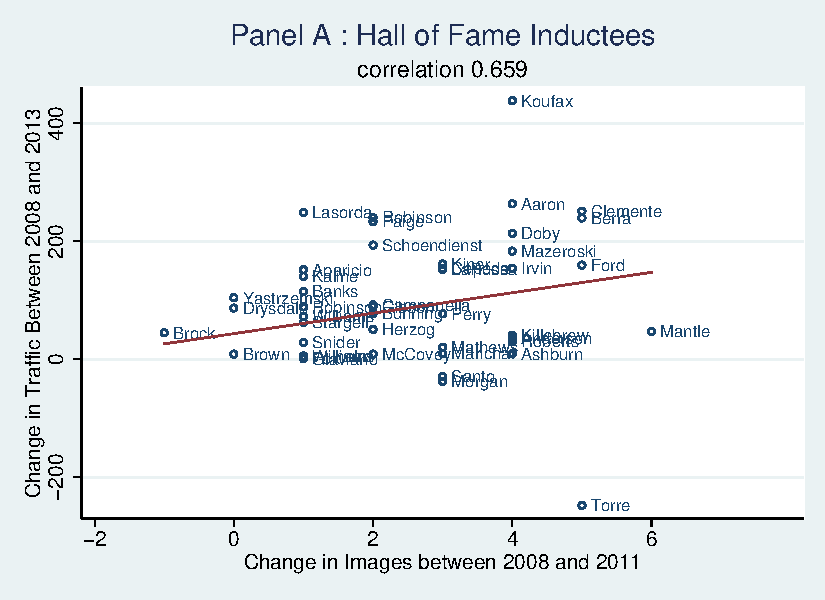
\includegraphics[scale=0.80]{../tables/traf_scatter_1.pdf}\\
%% \vspace{5mm}
%% 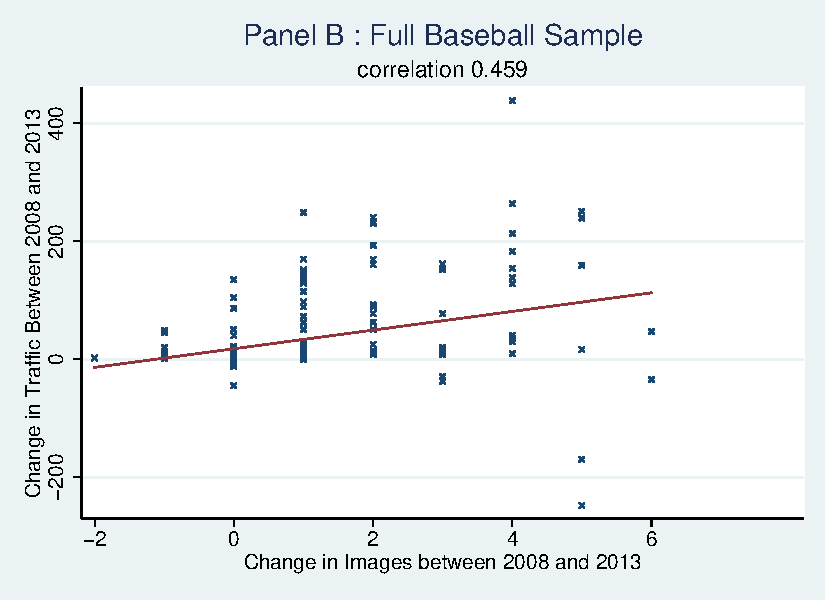
\includegraphics[scale=0.80]{../tables/traf_scatter_2.pdf}

%% \end{center}
%% \begin{quote}
%% \begin{adjustwidth}{-2cm}{-2cm}
%% \emph{Note:} This plot documents the relationship between the change in images for a given page before and after the digitization of Baseball Digest and associated change in traffic. Panel A, plots the data for all Hall-of-Fame players in the out-of-copyright group and each point is labeled with the player's last name. Panel B is a similar plot for all out-of-copyright baseball players. The correlation coefficient is about 0.659 for Hall of Fame players and 0.459 for the full sample. See text for more detailed data and variable descriptions.
%% \end{adjustwidth}
%% \end{quote}
%% \end{figure}

%%%%% NEXT APPENDIX

\newpage
\FloatBarrier

\subsection{Appendix A2 : Simple Theoretical Framework}
\label{sec:theory}

\label{sec:model}
This section builds a simple toy model to understand how copyright might affect the reuse of digitized information.

\subsection*{Setup}

Consider a wikipedia page $W_{q,k}$ for an item of quality $q$ and knowledge level $k$. The quality is a parameter that captures how inherently interesting a topic is, for example a famous, well-known baseball player will have higher $q$ than a less well-known player. Knowledge level $k$ captures how much information exists on a given page. Let $q \in \{0,\infty\}$ and $k \in \{{1}/{4},\infty\}$.

Now define value, $V(W_{q,k})=\sqrt{q}+\sqrt{k}-\frac{k}{4}$ to be the value that the Wikipedia community delivers from a page $W_{q,k}$.  In a context like Wikipedia, $V$ could be the traffic that a page receives for example. Note that while $\frac{dV}{dq}>0$ and $\frac{dV}{dk}>0$, $\frac{d^2V}{dq^2}<0$ and $\frac{d^2V}{dk^2}<0$. This simply implies diminishing but positive marginal returns from increased information and increased player quality to $V$.

Define $C(W_{q,k})=\frac{k}{q}$ to be the cost of adding $k$ units of information to a page with quality level $q$. Here, $\frac{dC}{dk}>0$ implying higher costs of information acquistion for higher levels of knowledge, but $\frac{dC}{dq}<0$ , implying that it is easier to source information for higher quality topics, presumably because such information is more easily available. 

Under this setup, the Wikipedia community solves the following, simple maximization problem to determine optimal levels of $k$, i.e. $k^*$

$$k^* = \max_k \Big[ V(W_{q,k}) - C(W_{q,k}) \Big]$$

$$k^* = \max_k \Big[\sqrt{q}+\sqrt{k}-\frac{k}{4} - k/q\Big]$$

$$k^* = \frac{4q^2}{(q+4)^2}$$

\subsection*{Digitization and Copyright}

Now consider that a digitization project makes it easier to access information to a certain topic, but that these reduction in costs depend on the copyright status of the underlying material. For topics that can benefit from out-of-copyright material, this reduction in cost is greater than it is for in-copyright material. A general way to parameterize this change is to assume that costs of adding information are reduced differentially for different copyright status groups.

\newpage

Accordingly, let $$C_{in-copy}(W_{q,k})=\frac{C(W_{q,k})}{2}=\frac{k}{2q}$$ $$C_{out-of-copy}(W_{q,k})=\frac{C(W_{q,k})}{4}=\frac{k}{4q}$$

Solving a similar maximization problem as before, we now obtain:

$$k^*_{in-copy}= \frac{4q^2}{(q+2)^2}$$

$$k^*_{out-of-copy}= \frac{4q^2}{(q+1)^2}$$

Therefore, $k^*_{out-of-copy}>k^*_{in-copy}>k^*$. This setup delivers the first two results that we obtained in the main part of the paper, i.e. digitization increased amount of information for both in-copyright and out-of-copyright pages, but this increase is significantly greater for out-of-copyright pages. 

\subsection*{Differential Effects for Images vs. Text}

While the previous section modeled the idea that copyright restrictions create differential cost reductions for digital information, the differential impact of copyright by media type were not discussed. However, while it is possible to paraphrase textual material without violating copyright, reusing copyrighted images without violating copyright is harder.

Accordingly, let

$$C^{images}_{in-copy}(W_{q,k})=C^{text}_{in-copy}(W_{q,k})=\frac{C(W_{q,k})}{2}=\frac{k}{2q}$$

$$C^{images}_{out-of-copy}(W_{q,k})=\frac{C(W_{q,k})}{4}=\frac{k}{4q}$$
$$C^{text}_{out-of-copy}(W_{q,k})=\frac{C(W_{q,k})}{2}=\frac{k}{2q}$$

Solving the maximization problem, we obtain:

$$k^{*text}_{out-of-copy}=k^{*text}_{in-copy}= \frac{4q^2}{(q+2)^2}$$

$$k^{*images}_{out-of-copy}= \frac{4q^2}{(q+1)^2} \hspace{5mm} \Big >  \hspace{5mm} k^{*images}_{in-copy}= \frac{4q^2}{(q+2)^2}$$

Therefore, as is clear from this simple example, the differential cost reductions for images and text provides a direct prediction: the impact of copyright on reducing information reuse is driven primarily by a difference in the reuse of images rather than the reuse of textual information. 


\subsection*{Differential Effects by Quality Levels}

Now consider the impact of the copyright law on affecting increase in knowledge for topics of different quality types.

For in-copyright topics, percent increase in knowledge $\Delta k_{in-copy}=\frac{k^*_{in-copy}-k^*}{k^*}$ and similarly, for out-of-copyright topics, $\Delta k_{out-of-copy}=\frac{k^*_{out-of-copy}-k^*}{k^*}$. Solving we get:

$$ \Delta k_{in-copy} = \frac{4q^2}{(q+4)^2} \Big[ \frac{4(q+3)}{(q+2)^2} \Big] $$

$$ \Delta k_{out-of-copy} = \frac{4q^2}{(q+4)^2} \Big[ \frac{3(2q+5)}{(q+1)^2} \Big] $$

$$ \therefore \Delta = \Delta k_{out-of-copy} - \Delta k_{in-of-copy} = \frac{4q^2 (2q+3)}{(q+1)^2(q+2)^2} $$

%%\Big[\frac{(q+4)^2(2q+3)}{(q+1)^2(q+2)^2} \Big]$$

$$ \therefore \frac{d\Delta}{dk} = - \Big[ \frac{8q(q^3-6q-6)}{(q+1)^3(q+2)^3} \Big] $$

%%  \frac{2(q+4)(q^3+12q^2+30q+22)}{(q+1)^3(q+2)^3}   $$
%% \implies \boxed{\Delta > 0} \hspace{5mm} and

$$ \implies \hspace{5mm} \boxed{\frac{d\Delta}{dq} > 0 \hspace{5mm} \forall q \in (0, \approx 2.84)}  \hspace{5mm} and \hspace{5mm} \boxed{\frac{d\Delta}{dq} < 0 \hspace{5mm} \forall q \in (\approx 2.84,\infty)}$$

Therefore, under this simple model, while the increase in information reuse is greater for out-of-copyright topics than for in-copyright topics at the same quality level, this magnitude of this positive effect depends significantly on the quality level $q$ of the topic. For low $q$ (i.e. $0<q<\approx2.84$), higher quality topics experience a greater increase in information reuse as compared to lower quality topics. The intuition for this effect is simple, returns to information are higher for higher quality topics, and therefore a greater reduction in cost of adding information due to a lack of copyright is most beneficial for these topics. However, after a certain threshold, this logic no longer applies, and an increase in topic quality reduces the benefit from out-of-copyright status. The intuition for this effect is the following: higher quality topics had higher levels of initial information, and returns to adding more information are decreasing. Therefore, it becomes more valuable to add information to lower quality topics because these have a lower starting starting point, as compared to adding information to topics that already have higher levels of information to begin with.

In this way -- the model builds intuition for the key results of the paper, (i) digitization improves the quality of Wikipedia information, (ii) Copyright law reduces the potential benefits from digitiziation (iii) copyright mainly operates through the reuse of images rather than text and (iv) Potential benefits from a lack of copyright on digital material are greatest for topics of ``intermediate'' quality. 

\begin{center}
\textbf{Fig: A plot of how $\Delta$ varies with $q$}
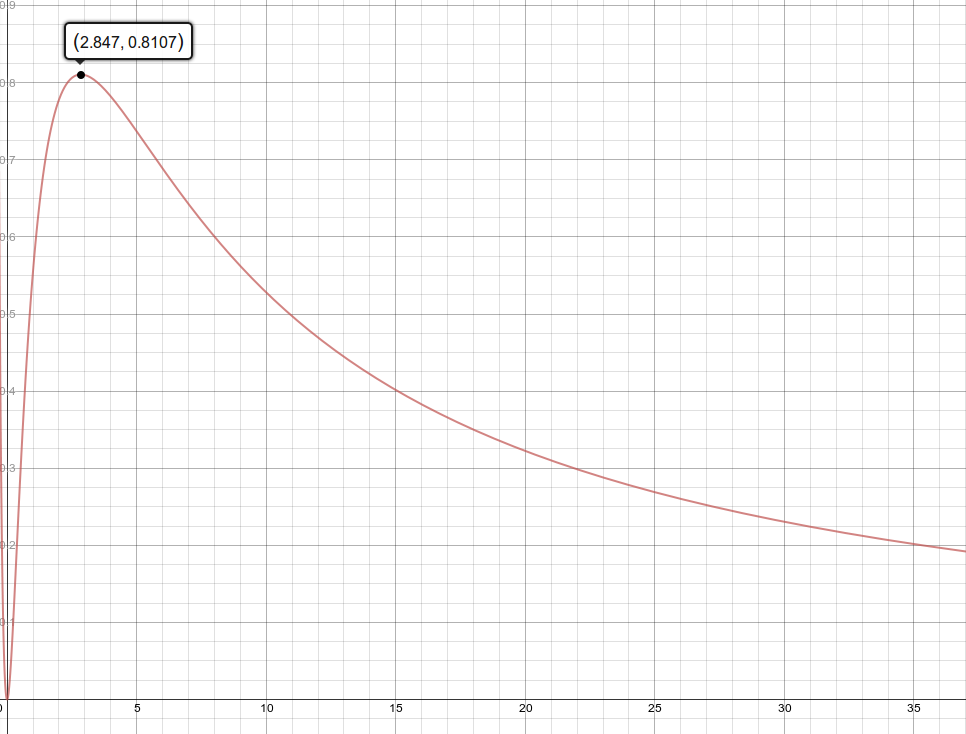
\includegraphics[scale = 0.3]{../tables/model.png}
\end{center}
  


%Now, for all $q \in \{0,\infy \}$, we have $\Delta k_{out-of-copy}>\Delta k_{in-copy}$










































\end{document}


%%% backup stuff


%% %%%%% COPY Table %%%%

%% \begin{center}
%% \begin{table}[!htbp]
%% %\caption{Impact of Copyright on Baseball Digest Reuse }
%% \caption{Difference-in-Difference Regressions Estimating Impact of 1964 Copyright Experiment on Wikipedia Pages (Sample B)}
%% %\caption{Difference-in-Difference Regressions Estimating Impact of Google Books Digitization Event on Baseball Wikipedia Pages}
%% \vspace{5mm}
%% {
\def\sym#1{\ifmmode^{#1}\else\(^{#1}\)\fi}
\begin{tabular*}{\hsize}{@{\hskip\tabcolsep\extracolsep\fill}l*{3}{c}}
\toprule
                                                  &\multicolumn{1}{c}{OLS}&\multicolumn{1}{c}{OLS}&\multicolumn{1}{c}{Log-OLS}\\
\midrule \vspace{5mm} \makebox[13em][l]{\underline{\textbf{Panel A : Images}}\vspace{5mm} ($\bar{y}$=0.66)}\\
\emph{out-of-copy X post}                         &       0.280         &       0.226         &      0.0646         \\
                                                  &     (0.106)\sym{***}&     (0.105)\sym{**} &    (0.0352)\sym{*}  \\

\end{tabular*} }
{
\def\sym#1{\ifmmode^{#1}\else\(^{#1}\)\fi}
\begin{tabular*}{\hsize}{@{\hskip\tabcolsep\extracolsep\fill}l*{3}{c}}
\midrule \vspace{5mm} \makebox[13em][l]{\underline{\textbf{Panel B : Text}}\vspace{5mm} ($\bar{y}$=1179.96)}\\
\emph{out-of-copy X post}                         &       234.9         &       205.9         &     -0.0466         \\
                                                  &     (96.06)\sym{**} &     (98.08)\sym{**} &    (0.0955)         \\
\midrule
Player-Page FE                                    &         Yes         &         Yes         &         Yes         \\
Time FE                                           &        Year         &Quality X Year         &        Year         \\
N                                                 &        4869         &        4869         &        4869         \\
Adj R-square                                      &       0.397         &       0.404         &       0.613         \\
\bottomrule
\end{tabular*}
}

%% \begin{quote}
%% \vspace{5mm}

%% \emph{+:p$<$0.15; *:p$<$0.10; **:p$<$0.05; ***:p$<$0.01 
%% \newline
%% Standard errors clustered at player-page-level shown in parentheses.}

%% \vspace{5mm}

%% \emph{Note:} This regression estimates the likelihood of citation on baseball player Wikipedia pages to Baseball Digest magazine for out-of-copyright players (debut before 1964) as compared to in-copyright players (debut on or after 1964), before and after the digitization of the magazine by Google Books.
%% \vspace{5mm}

%% Specification: $Y_{it} = \alpha + \beta_1 \times post_t \times out-of-copy_i + \gamma_i+ \delta_t + \epsilon_{it}$ where $\gamma_{i}$ and $\delta_{t}$ represents player-page and calendar-year fixed effects respectively for player-page $i$  and calendar-year $t$.  \emph{post}:0/1,=1 if year is greater than 2008 and \emph{out-of-copy}:0/1,=1 if player debut before 1964. All models include calendar year fixed effects. Columns (1) and (2) estimate OLS models, with column (2) also including player-page level fixed effects. Column (3) estimates Log-OLS models (i.e. the dependent variable is Log(Y+1)) with player-page and calendar-year fixed effects. See text for detailed data and variable descriptions.

%% %\emph{Decade}, indicator variables for decade of player debut. \emph{Quality}, indicator variables for percentile rank of player in cohort based on sport-specific covariates.

%% %%Column (1) includes \emph{controls}, proxying for a player's \emph{quality} rank based on sport-specific covariates.

%% \end{quote}
%% \label{tab:copy_b}
%% \end{table}
%% \end{center}


%% %%%%% DDD Table %%%%

%% \begin{center}
%% \begin{table}[!htbp]
%% \caption{DDD Regressions Estimating Impact of 1964 Copyright Experiment on Baseball Wikipedia Pages using Basketball Pages as 2nd set of Controls}
%% \vspace{5mm}
%% {
\def\sym#1{\ifmmode^{#1}\else\(^{#1}\)\fi}
\begin{tabular*}{\hsize}{@{\hskip\tabcolsep\extracolsep\fill}l*{3}{c}}
\toprule
            &\multicolumn{1}{c}{(1)}&\multicolumn{1}{c}{(2)}&\multicolumn{1}{c}{(3)}\\
            &\multicolumn{1}{c}{Citations}&\multicolumn{1}{c}{Images}&\multicolumn{1}{c}{Text}\\
\midrule
\emph{out-of-copy X post X baseball}&       0.215         &       0.375         &       191.8         \\
            &     (0.112)\sym{*}  &     (0.156)\sym{**} &     (180.8)         \\
\addlinespace
\emph{out-of-copy X post}&   -1.74e-14         &      0.0667         &       126.0         \\
            &  (5.94e-09)         &    (0.0915)         &     (137.9)         \\
\addlinespace
\emph{baseball X post}&       0.275         &       0.361         &       298.0         \\
            &    (0.0562)\sym{***}&    (0.0664)\sym{***}&     (66.68)\sym{***}\\
\midrule
Player FE   &         Yes         &         Yes         &         Yes         \\
Time FE     &        Year         &        Year         &        Year         \\
adj. $R^2$  &      0.0775         &       0.197         &       0.410         \\
N           &       14365         &       14365         &       14365         \\
Clusters    &        1105         &        1105         &        1105         \\
\bottomrule
\end{tabular*}
}

%% \begin{quote}
%% \vspace{5mm}
%% \emph{+:p$<$0.15; *:p$<$0.10; **:p$<$0.05; ***:p$<$0.01 
%% \newline
%% Standard errors clustered at player-level shown in parentheses.}
%% \vspace{5mm}


%% \emph{Note:} Page-year level observations for full sample. \emph{out-of-copy}: 0/1, =1 for players making debut before 1964. \emph{baseball}:0/1,  =1 for baseball players and =0 for basketball players. \emph{post}:0/1,=1 if year is greater than 2008. 

%% Specification: $Y_{itg} = \alpha + \beta_1 \times out-of-copy_i \times post_t \times baseball_g + \beta_2 \times out-of-copy_i \times post_t + \beta_3 \times baseball_g \times post_t + \gamma_i + \delta_t + \epsilon_{igt}$

%% for player $i$ in year $t$ and in sport $g$ where $\gamma_{i}$ and $\delta_t$ represents player and time fixed effects respectively.  All estimates are from ordinary-least-squares (OLS) models. See text for detailed data and variable descriptions.

%% \end{quote}
%% \label{tab:ddd}
%% \end{table}
%% \end{center}


%% %%%%%%%%%%%%% IVREG
%% \newpage
%% \begin{center}
%% \begin{table}[!htbp]

%% \caption{Is an Increase in Images Associated With an Increase in Traffic?}
%% \vspace{5mm}
%% \begin{adjustwidth}{0.5cm}{}
%% {
\def\sym#1{\ifmmode^{#1}\else\(^{#1}\)\fi}
\begin{tabular}{l*{6}{c}}
\toprule
                    &\multicolumn{2}{c}{OLS}                    &\multicolumn{2}{c}{First Stage}            &\multicolumn{2}{c}{IV Estimates}           \\\cmidrule(lr){2-3}\cmidrule(lr){4-5}\cmidrule(lr){6-7}
                    &\multicolumn{1}{c}{(1)}&\multicolumn{1}{c}{(2)}&\multicolumn{1}{c}{(3)}&\multicolumn{1}{c}{(4)}&\multicolumn{1}{c}{(5)}&\multicolumn{1}{c}{(6)}\\
                    &\multicolumn{1}{c}{Traffic}&\multicolumn{1}{c}{Traffic}&\multicolumn{1}{c}{Images}&\multicolumn{1}{c}{Images}&\multicolumn{1}{c}{Traffic}&\multicolumn{1}{c}{Traffic}\\
\midrule
Images              &       122.0\sym{***}&       44.38\sym{*}  &                     &                     &       88.55\sym{***}&       113.8\sym{**} \\
                    &     (34.91)         &     (23.73)         &                     &                     &     (31.62)         &     (45.21)         \\
\addlinespace
Out-Of-Copy. X Post &                     &                     &       0.609\sym{***}&       0.274\sym{***}&                     &                     \\
                    &                     &                     &     (0.154)         &    (0.0964)         &                     &                     \\
\midrule
Controls            &         Yes         &   Player FE         &         Yes         &   Player FE         &         Yes         &   Player FE         \\
Year FE             &         Yes         &         Yes         &         Yes         &         Yes         &         Yes         &         Yes         \\
N                   &        3787         &        3787         &        3787         &        3787         &        3787         &        3787         \\
adj. $R^2$          &       0.446         &      0.0737         &      0.0644         &       0.190         &       0.415         &     -0.0366         \\
F-Stat              &                     &                     &       15.62         &        8.07         &                     &                     \\
\bottomrule
\multicolumn{7}{l}{\footnotesize }\\
\multicolumn{7}{l}{\footnotesize }\\
\end{tabular}
}

%% \end{adjustwidth}

%% \begin{quote}
%% \emph{+:p$<$0.15; *:p$<$0.10; **:p$<$0.05; ***:p$<$0.01 
%% \newline
%% Standard errors clustered at player-level shown in parentheses.}
%% \vspace{5mm}

%% \emph{Note:} Page-year level observations for sample of baseball players. \emph{Images} measures number of images on player-page in a given year. 
%% All estimates are from ordinary-least-squares (OLS) models. Specification for Columns (1) is $Y_{i} = \alpha + \beta_1 \cdot Images_{it} +\delta_t + \epsilon_{it}$, while Column (2) adds individual player dummies. 

%% Columns (3-6) present results from IV estimation, with and without player fixed effects. See text for detailed data and variable descriptions.

%% \end{quote}
%% \label{tab:ivreg}
%% \end{table}
%% \end{center}


%% OLD APPENDIXES

%% \subsection{Appendix A1 : The 1964 Copyright Experiment}
%% \label{sec:enclosure}

%% Legal opinion about copyright law concerning periodicals (under the Copyright Act of 1909) from University of Pennsylvania Libraries is reproduced below for reference. See \url{http://onlinebooks.library.upenn.edu/cce/firstperiod.html} for more details.

%% \begin{quotation}
%% For works that received their copyright before 1978, a renewal had to be filed in the work's 28th year with the Library of Congress Copyright Office for its term of protection to be extended. The need for renewal was eliminated by the Copyright Renewal Act of 1992, but works that had already entered the public domain by non-renewal did not regain copyright protection. Therefore, works published before 1964 that were not renewed are in the public domain. With rare exception (such as very old works first published after 2002) no additional copyrights will expire (thus entering the public domain) until at least 2019 due to changes in the applicable laws.
%% \end{quotation}

%% The following screenshot is from a Wikipedia banner explaining the legal use of an image sourced from Baseball Digest.

%% \begin{figure}[!htbp]
%% \centering
%% 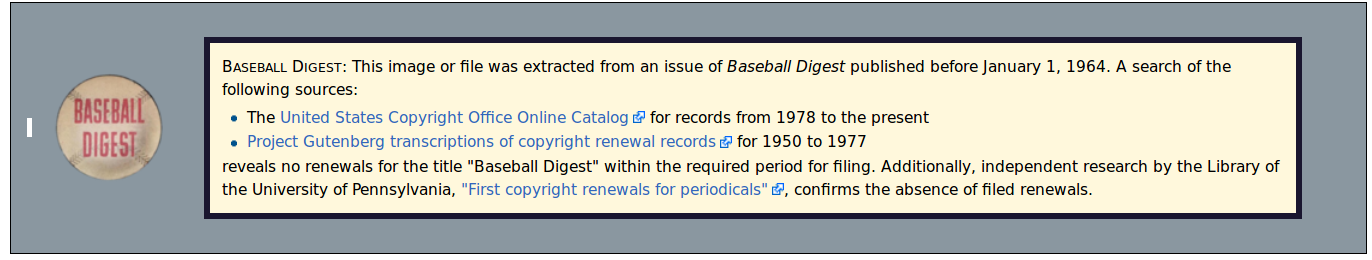
\includegraphics[scale = 0.3]{../tables/bd_copyrightcaption.png}
%% \caption*{A screenshot from Wikipedia explaining copyright law pertaining to reuse of material from Baseball Digest}
%% \label{fig:copyrightcaption}
%% \end{figure}

%% \newpage

%% \subsection{Appendix A2 : Back-of-the-Envelope Welfare Calculation}
%% \label{sec:envelope}

%% This section outlines the methodology through which I arrive at my estimate of about \$372,920 annually for a lower bound on the loss to social welfare from copyright.

%% In order to arrive at this estimate two pieces of data are needed: (a) the approximate value of a page-view to society and (b) estimated page-views lost due to copyright. For piece (a) I used \url{webindetail.com} which provides the estimated daily earnings of Wikipedia from potential advertising which would equal to \$2.2 million dollars daily for about 400 million daily page-views.\footnote{While Wikipedia does not accept advertising, \url{webindetail.com} arrives at this estimate based on a comparables analysis based on other similar websites with a comparable user base.} This translates into a value to Wikipedia of about \$0.0055 per page-view from advertising. For piece (b) results from this study suggest that for every missing image, a Wikipedia page receives about 88 fewer page-views per month (Table \ref{tab:ivreg}) and that pages have 0.315 fewer images on average (Table \ref{tab:ddd}) due to copyright. Therefore, a page affected by copyright is expected to lose about \$0.152 per month. For the set of 335 pages affected by copyright in this study. This translates into an annual loss of about \$612 or a net present value of about \$30,600.\footnote{discounted at a rate of 2\% per year over a perpetual life term} Assuming that about 5\% of all 4.1 million articles on Wikipedia are affected in a similar way, this translates into an annual loss of about \$372,920 or a net present value of about \$18.69 million. These estimates are economically significant for Wikipedia in the light of estimates of the economic value of Wikipedia itself which is about \$43.5 million per year \citep{greenstein_technology:_2013}. Further, these estimates represent only a lower bound on lost surplus because advertising rates capture only the valuation advertisers place on readers and do not calculate value to readers including value of derivative works of Wikipedia pages.

%% \newpage


